% =====================================================================
%  Condensed crystal graphs — three ABO3 materials (figure BODY)
% ---------------------------------------------------------------------
%  Preamble-free fragment (same pattern as gps_encoder_fig.tex and
%  pretraining_transfer_fig.tex): \input this from the paper inside a
%  figure environment; compile graph_construction.tex for a standalone
%  preview PDF.  Everything below (colors, styles, the loop macro, the
%  tikzpicture) is legal in the document body and is wrapped in a group
%  so nothing leaks into the main document.
%
%     % main-doc preamble:
%     \usepackage{tikz}
%     \usetikzlibrary{positioning,arrows.meta,calc,backgrounds}
%
%     % main-doc body (full text width -- the 3x3 grid is unreadable at
%     % single-column width):
%     \begin{figure*}[t]
%       \centering
%       \resizebox{\textwidth}{!}{% =====================================================================
%  Condensed crystal graphs — three ABO3 materials (figure BODY)
% ---------------------------------------------------------------------
%  Preamble-free fragment (same pattern as gps_encoder_fig.tex and
%  pretraining_transfer_fig.tex): \input this from the paper inside a
%  figure environment; compile graph_construction.tex for a standalone
%  preview PDF.  Everything below (colors, styles, the loop macro, the
%  tikzpicture) is legal in the document body and is wrapped in a group
%  so nothing leaks into the main document.
%
%     % main-doc preamble:
%     \usepackage{tikz}
%     \usetikzlibrary{positioning,arrows.meta,calc,backgrounds}
%
%     % main-doc body (full text width -- the 3x3 grid is unreadable at
%     % single-column width):
%     \begin{figure*}[t]
%       \centering
%       \resizebox{\textwidth}{!}{% =====================================================================
%  Condensed crystal graphs — three ABO3 materials (figure BODY)
% ---------------------------------------------------------------------
%  Preamble-free fragment (same pattern as gps_encoder_fig.tex and
%  pretraining_transfer_fig.tex): \input this from the paper inside a
%  figure environment; compile graph_construction.tex for a standalone
%  preview PDF.  Everything below (colors, styles, the loop macro, the
%  tikzpicture) is legal in the document body and is wrapped in a group
%  so nothing leaks into the main document.
%
%     % main-doc preamble:
%     \usepackage{tikz}
%     \usetikzlibrary{positioning,arrows.meta,calc,backgrounds}
%
%     % main-doc body (full text width -- the 3x3 grid is unreadable at
%     % single-column width):
%     \begin{figure*}[t]
%       \centering
%       \resizebox{\textwidth}{!}{% =====================================================================
%  Condensed crystal graphs — three ABO3 materials (figure BODY)
% ---------------------------------------------------------------------
%  Preamble-free fragment (same pattern as gps_encoder_fig.tex and
%  pretraining_transfer_fig.tex): \input this from the paper inside a
%  figure environment; compile graph_construction.tex for a standalone
%  preview PDF.  Everything below (colors, styles, the loop macro, the
%  tikzpicture) is legal in the document body and is wrapped in a group
%  so nothing leaks into the main document.
%
%     % main-doc preamble:
%     \usepackage{tikz}
%     \usetikzlibrary{positioning,arrows.meta,calc,backgrounds}
%
%     % main-doc body (full text width -- the 3x3 grid is unreadable at
%     % single-column width):
%     \begin{figure*}[t]
%       \centering
%       \resizebox{\textwidth}{!}{\input{figures/graph_construction_fig}}
%       \caption{Condensed crystal graphs of three $ABO_3$ compounds:
%         cubic perovskite SrTiO$_3$ (mp-5229), orthorhombically
%         distorted perovskite GdFeO$_3$ (mp-600576) and ilmenite
%         FeTiO$_3$ (mp-19417); $t$ is the Goldschmidt tolerance factor.
%         (a)~Schematic unit cells.  (b)~Bonding edges and
%         (c)~polyhedral edges of the crystal graph, condensed by
%         symmetry: one node per symmetry-inequivalent site and one
%         drawn edge per symmetry class of edges; loops denote sharing
%         between symmetry-equivalent sites.  $\times N$ on an edge is
%         the number of bonds of that class per cation, $\times N$ under
%         a node the number of such sites per formula unit.  All three
%         graphs share the $B$--O core bonding motif, and the distortion
%         of GdFeO$_3$ appears as split core/extended Gd--O bond classes.
%         Polyhedral edges separate the structure types: both
%         perovskites carry the $B$--$B$ corner-sharing loop, whereas
%         ilmenite has no like-cation corner sharing -- its cations form
%         edge-sharing layers linked by Fe--Ti face sharing.}
%       \label{fig:graph-construction}
%     \end{figure*}
%
%  Content: all graph content is EXTRACTED from the real v4 builder
%  output (build_crystal_graph_from_structure on MP structures mp-5229 /
%  mp-600576 / mp-19417, node orbits by SpacegroupAnalyzer) — one node
%  per symmetry-inequivalent site, one drawn edge per symmetry class.
%  Layout: 3x3 grid, materials as columns, rows (top -> bottom)
%    (a) structure motif (3-D ball-and-stick cells; GENERATED by
%        gen_motif3d.py — edit that script, not the Row-1 block)
%    (b) bonding edges   (core solid / extended dashed)
%    (c) polyhedral edges (corner / edge / face / 4+ sharing)
%  Story: both perovskites share the B-B corner-sharing loop; ilmenite
%  has NO like-cation corner sharing (edge loops + Fe-Ti face sharing).
%  Native size ~17.4 x 11.7 cm (aspect 1.5) so that at \textwidth of a
%  two-column page the \scriptsize labels stay ~7 pt.
%  Palette/styles match gps_encoder_fig.tex.
% =====================================================================
\begingroup

% ---- palette (shared with gps_encoder_fig.tex) ----------------------
\definecolor{Bcol}{HTML}{4C72B0}    % B-site / metal cation
\definecolor{Ocol}{HTML}{C44E52}    % anion (oxygen)
\definecolor{Acol}{HTML}{55A868}    % A-site large cation
\definecolor{panel}{HTML}{EEF1F6}   % light panel fill
\definecolor{ink}{HTML}{2B2B2B}
% polyhedral-edge classes (colorblind-safe, echoes the old blue/orange/red/purple)
\definecolor{cCorner}{HTML}{0077BB}
\definecolor{cEdge}{HTML}{EE7733}
\definecolor{cFace}{HTML}{CC3311}
\definecolor{cMulti}{HTML}{AA4499}

% ---- shared styles (local to this group) ----------------------------
\tikzset{
  siteA/.style={circle, draw=ink, thick, fill=Acol, minimum size=7.4mm,
                inner sep=0pt, font=\small\bfseries\sffamily, text=white},
  siteB/.style={circle, draw=ink, thick, fill=Bcol, minimum size=7.4mm,
                inner sep=0pt, font=\small\bfseries\sffamily, text=white},
  siteO/.style={circle, draw=ink, thick, fill=Ocol, minimum size=7.4mm,
                inner sep=0pt, font=\small\bfseries\sffamily, text=white},
  core/.style={line width=1.6pt, gray!55!black},
  ext/.style={line width=1.3pt, gray!55!black, dash pattern=on 3.2pt off 2.4pt},
  pcorner/.style={line width=1.5pt, cCorner},
  pedge/.style={line width=1.5pt, cEdge},
  pface/.style={line width=1.5pt, cFace},
  pmulti/.style={line width=1.5pt, cMulti},
  panelbox/.style={draw=ink!55, rounded corners=4pt, fill=panel},
  ptitle/.style={font=\bfseries\sffamily, text=ink},
  psub/.style={font=\scriptsize\sffamily, text=ink!75},
  rowlbl/.style={font=\bfseries\sffamily, text=ink, anchor=west},
  leglbl/.style={font=\scriptsize\sffamily, text=ink, anchor=west},
  leghint/.style={font=\scriptsize\sffamily, text=ink!60, anchor=north west,
                  text width=36mm, align=left, inner sep=0pt},
  % motif ingredients (ball-and-stick, matching the gps_encoder structure panel;
  % sizes keep gps_encoder's atom/spacing ratio at this row's 1.0 grid spacing)
  matomA/.style={circle, draw=ink, line width=0.7pt, fill=Acol, minimum size=5.0mm, inner sep=0pt},
  matomB/.style={circle, draw=ink, line width=0.7pt, fill=Bcol, minimum size=3.8mm, inner sep=0pt},
  matomO/.style={circle, draw=ink, line width=0.7pt, fill=Ocol, minimum size=2.8mm, inner sep=0pt},
  mbond/.style={line width=1.2pt, gray!60!black},
  medge/.style={line width=0.6pt, ink!40},
}

% loop macro: \gcloop{style}{node}{center direction in deg}
% \providecommand (not \newcommand): inert if the main doc, or a second
% \input of this fragment, already defined it.
\providecommand{\gcloop}[3]{%
  \path[#1] (#2) edge[out=#3+26, in=#3-26, looseness=6, min distance=6mm] (#2);}

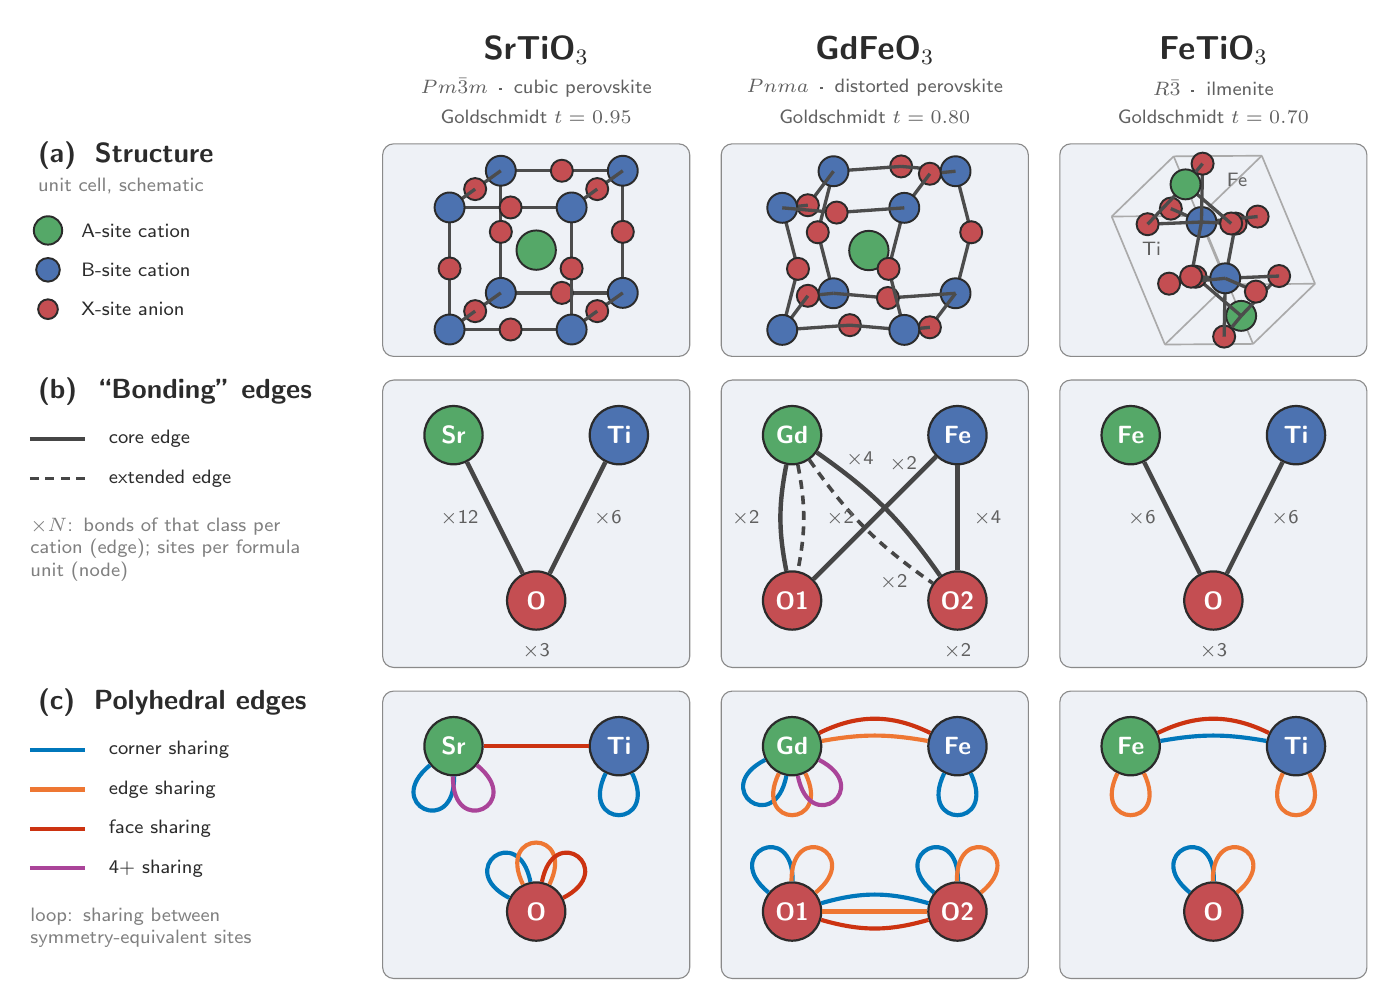
\begin{tikzpicture}

% =====================================================================
%  Geometry bookkeeping (cm)
%    legend column at x = -4.85 .. -0.7 ; material columns at
%    x0 = 0, 4.3, 8.6 ; panel x = x0-0.35 .. x0+3.55 (inner width 3.9)
%  Rows (absolute y):  header 10.55 / 10.91 / 11.38 ;
%    (a) motif    7.50 .. 10.20   (scope shift y = 7.65)
%    (b) bonding  3.55 ..  7.20   (scope shift y = 3.95)
%    (c) poly    -0.40 ..  3.25   (scope shift y = 0)
%  Row (b)/(c) graph panels share one node layout: cations top
%  (y = 2.55), anions bottom (y = 0.45), so the eye maps nodes across rows.
% =====================================================================

% ---------------------------------------------------------------------
%  Column headers
% ---------------------------------------------------------------------
\foreach \x/\formula/\proto/\tf in {%
    1.6/{SrTiO$_3$}/{$Pm\bar3m$ \,·\, cubic perovskite}/{0.95},
    5.9/{GdFeO$_3$}/{$Pnma$ \,·\, distorted perovskite}/{0.80},
    10.2/{FeTiO$_3$}/{$R\bar3$ \,·\, ilmenite}/{0.70}}{
  \node[ptitle, font=\large\bfseries\sffamily] at (\x,11.38) {\formula};
  \node[psub] at (\x,10.91) {\proto};
  \node[psub] at (\x,10.55) {Goldschmidt $t=\tf$};
}

% ---------------------------------------------------------------------
%  Row 1 — structure motifs (3-D ball-and-stick, oblique projection;
%  GENERATED by gen_motif3d.py (this directory) — edit that script, not this block)
% ---------------------------------------------------------------------
% SrTiO3: cubic cell, straight B-O-B cage, A at body centre
\begin{scope}[shift={(0,7.65)}]
  \draw[panelbox] (-0.35,-0.15) rectangle (3.55,2.55);
  \draw[mbond] (1.151,0.657) -- (1.926,0.657);
  \draw[mbond] (1.926,0.657) -- (2.700,0.657);
  \draw[mbond] (1.151,2.208) -- (1.926,2.208);
  \draw[mbond] (1.926,2.208) -- (2.700,2.208);
  \draw[mbond] (1.151,0.657) -- (1.151,1.432);
  \draw[mbond] (1.151,1.432) -- (1.151,2.208);
  \draw[mbond] (2.700,0.657) -- (2.700,1.432);
  \draw[mbond] (2.700,1.432) -- (2.700,2.208);
  \node[matomO] at (1.926,0.657) {};
  \node[matomO] at (1.926,2.208) {};
  \node[matomO] at (1.151,1.432) {};
  \node[matomO] at (2.700,1.432) {};
  \node[matomB] at (1.151,0.657) {};
  \node[matomB] at (1.151,2.208) {};
  \node[matomB] at (2.700,0.657) {};
  \node[matomB] at (2.700,2.208) {};
  \draw[mbond] (0.825,0.425) -- (1.151,0.657);
  \draw[mbond] (2.375,0.425) -- (2.700,0.657);
  \draw[mbond] (0.825,1.975) -- (1.151,2.208);
  \draw[mbond] (2.375,1.975) -- (2.700,2.208);
  \node[matomO] at (0.825,0.425) {};
  \node[matomO] at (2.375,0.425) {};
  \node[matomO] at (0.825,1.975) {};
  \node[matomO] at (2.375,1.975) {};
  \node[matomA] at (1.600,1.200) {};
  \draw[mbond] (0.500,0.192) -- (0.825,0.425);
  \draw[mbond] (2.050,0.192) -- (2.375,0.425);
  \draw[mbond] (0.500,1.742) -- (0.825,1.975);
  \draw[mbond] (2.050,1.742) -- (2.375,1.975);
  \draw[mbond] (0.500,0.192) -- (1.275,0.192);
  \draw[mbond] (1.275,0.192) -- (2.050,0.192);
  \draw[mbond] (0.500,1.742) -- (1.275,1.742);
  \draw[mbond] (1.275,1.742) -- (2.050,1.742);
  \draw[mbond] (0.500,0.192) -- (0.500,0.967);
  \draw[mbond] (0.500,0.967) -- (0.500,1.742);
  \draw[mbond] (2.050,0.192) -- (2.050,0.967);
  \draw[mbond] (2.050,0.967) -- (2.050,1.742);
  \node[matomO] at (1.275,0.192) {};
  \node[matomO] at (1.275,1.742) {};
  \node[matomO] at (0.500,0.967) {};
  \node[matomO] at (2.050,0.967) {};
  \node[matomB] at (0.500,0.192) {};
  \node[matomB] at (0.500,1.742) {};
  \node[matomB] at (2.050,0.192) {};
  \node[matomB] at (2.050,1.742) {};
\end{scope}
% GdFeO3: edge O tangentially displaced (octahedral tilt)
\begin{scope}[shift={(4.3,7.65)}]
  \draw[panelbox] (-0.35,-0.15) rectangle (3.55,2.55);
  \node[matomO] at (1.935,2.263) {};
  \draw[mbond] (1.076,2.202) -- (1.935,2.263);
  \draw[mbond] (1.935,2.263) -- (2.626,2.202);
  \draw[mbond] (1.076,0.652) -- (0.876,1.427);
  \draw[mbond] (0.876,1.427) -- (1.076,2.202);
  \draw[mbond] (2.626,0.652) -- (2.825,1.427);
  \draw[mbond] (2.825,1.427) -- (2.626,2.202);
  \node[matomO] at (0.876,1.427) {};
  \node[matomO] at (2.825,1.427) {};
  \node[matomB] at (1.076,0.652) {};
  \node[matomB] at (1.076,2.202) {};
  \node[matomB] at (2.626,0.652) {};
  \node[matomB] at (2.626,2.202) {};
  \draw[mbond] (1.076,0.652) -- (1.767,0.592);
  \draw[mbond] (1.767,0.592) -- (2.626,0.652);
  \node[matomO] at (1.767,0.592) {};
  \draw[mbond] (0.750,0.620) -- (1.076,0.652);
  \draw[mbond] (2.300,0.220) -- (2.626,0.652);
  \draw[mbond] (0.750,1.770) -- (1.076,2.202);
  \draw[mbond] (2.300,2.170) -- (2.626,2.202);
  \node[matomO] at (0.750,0.620) {};
  \node[matomO] at (2.300,0.220) {};
  \node[matomO] at (0.750,1.770) {};
  \node[matomO] at (2.300,2.170) {};
  \node[matomA] at (1.525,1.195) {};
  \draw[mbond] (0.425,0.187) -- (0.750,0.620);
  \draw[mbond] (1.975,0.187) -- (2.300,0.220);
  \draw[mbond] (0.425,1.737) -- (0.750,1.770);
  \draw[mbond] (1.975,1.737) -- (2.300,2.170);
  \node[matomO] at (1.284,0.247) {};
  \draw[mbond] (0.425,0.187) -- (1.284,0.247);
  \draw[mbond] (1.284,0.247) -- (1.975,0.187);
  \draw[mbond] (0.425,0.187) -- (0.625,0.962);
  \draw[mbond] (0.625,0.962) -- (0.425,1.737);
  \draw[mbond] (1.975,0.187) -- (1.775,0.962);
  \draw[mbond] (1.775,0.962) -- (1.975,1.737);
  \node[matomO] at (0.625,0.962) {};
  \node[matomO] at (1.775,0.962) {};
  \node[matomB] at (0.425,0.187) {};
  \node[matomB] at (0.425,1.737) {};
  \node[matomB] at (1.975,0.187) {};
  \node[matomB] at (1.975,1.737) {};
  \draw[mbond] (0.425,1.737) -- (1.116,1.677);
  \draw[mbond] (1.116,1.677) -- (1.975,1.737);
  \node[matomO] at (1.116,1.677) {};
\end{scope}
% FeTiO3: primitive rhombohedral cell, oblique view (orientation
% sweep option Q): the two face-sharing Fe-Ti pairs along the body
% diagonal with the shared O3 triangles shown in depth
\begin{scope}[shift={(8.6,7.65)}]
  \draw[panelbox] (-0.35,-0.15) rectangle (3.55,2.55);
  \draw[medge] (2.104,0.009) -- (2.891,0.773);
  \draw[medge] (2.104,0.009) -- (0.985,0.001);
  \draw[medge] (2.104,0.009) -- (1.427,1.635);
  \draw[medge] (2.891,0.773) -- (1.773,0.765);
  \draw[medge] (2.891,0.773) -- (2.215,2.399);
  \draw[medge] (0.985,0.001) -- (1.773,0.765);
  \draw[medge] (0.985,0.001) -- (0.309,1.627);
  \draw[medge] (1.427,1.635) -- (2.215,2.399);
  \draw[medge] (1.427,1.635) -- (0.309,1.627);
  \draw[medge] (1.773,0.765) -- (1.096,2.391);
  \draw[medge] (2.215,2.399) -- (1.096,2.391);
  \draw[medge] (0.309,1.627) -- (1.096,2.391);
  \node[matomA, minimum size=3.8mm] at (1.953,0.365) {};
  \draw[mbond] (1.953,0.365) -- (2.435,0.871);
  \node[matomO] at (2.435,0.871) {};
  \draw[mbond] (1.953,0.365) -- (1.374,0.862);
  \node[matomO] at (1.374,0.862) {};
  \draw[mbond] (1.953,0.365) -- (1.737,0.102);
  \draw[mbond] (1.751,0.842) -- (2.435,0.871);
  \draw[mbond] (1.751,0.842) -- (1.374,0.862);
  \node[matomO] at (1.883,1.537) {};
  \draw[mbond] (1.751,0.842) -- (1.883,1.537);
  \node[matomO] at (1.737,0.102) {};
  \draw[mbond] (1.751,0.842) -- (1.737,0.102);
  \node[matomB] at (1.751,0.842) {};
  \draw[mbond] (1.751,0.842) -- (2.140,0.673);
  \draw[mbond] (1.751,0.842) -- (1.038,0.774);
  \node[matomO] at (2.140,0.673) {};
  \node[matomO] at (1.038,0.774) {};
  \node[matomO] at (2.162,1.626) {};
  \node[matomO] at (1.060,1.727) {};
  \draw[mbond] (1.449,1.557) -- (2.162,1.626);
  \draw[mbond] (1.449,1.557) -- (1.060,1.727);
  \node[matomB] at (1.449,1.557) {};
  \draw[mbond] (1.449,1.557) -- (1.463,2.298);
  \node[matomO] at (1.463,2.298) {};
  \draw[mbond] (1.449,1.557) -- (1.317,0.863);
  \node[matomO] at (1.317,0.863) {};
  \draw[mbond] (1.449,1.557) -- (1.826,1.538);
  \draw[mbond] (1.449,1.557) -- (0.765,1.529);
  \draw[mbond] (1.247,2.035) -- (1.463,2.298);
  \node[matomO] at (1.826,1.538) {};
  \draw[mbond] (1.247,2.035) -- (1.826,1.538);
  \node[matomO] at (0.765,1.529) {};
  \draw[mbond] (1.247,2.035) -- (0.765,1.529);
  \node[matomA, minimum size=3.8mm] at (1.247,2.035) {};
  \node[psub, anchor=west] at (-0.457+2.104,2.086+0.009) {Fe};
  \node[psub, anchor=east] at (-1.045+2.104,1.208+0.009) {Ti};
\end{scope}

% ---------------------------------------------------------------------
%  Row 2 — bonding edges (condensed graphs)
%  node layout: cations top, anions bottom (identical in row 3)
% ---------------------------------------------------------------------
% ---- SrTiO3 : Sr-O core, Ti-O core ----------------------------------
\begin{scope}[shift={(0,3.95)}]
  \draw[panelbox] (-0.35,-0.40) rectangle (3.55,3.25);
  \node[siteA] (Sr) at (0.55,2.55) {Sr};
  \node[siteB] (Ti) at (2.65,2.55) {Ti};
  \node[siteO] (O)  at (1.60,0.45) {O};
  \draw[core] (Sr) -- (O);
  \draw[core] (Ti) -- (O);
  % bond multiplicities (bonds of this class per cation; builder mp-5229)
  \node[psub, anchor=east] at (0.99,1.50) {$\times$12};
  \node[psub, anchor=west] at (2.21,1.50) {$\times$6};
  % site multiplicity: 3 equivalent O per formula unit
  \node[psub, anchor=north] at (1.60,0.02) {$\times$3};
\end{scope}
% ---- GdFeO3 : Fe-O1, Fe-O2 core ; Gd-O1, Gd-O2 core+extended --------
\begin{scope}[shift={(4.3,3.95)}]
  \draw[panelbox] (-0.35,-0.40) rectangle (3.55,3.25);
  \node[siteA] (Gd) at (0.55,2.55) {Gd};
  \node[siteB] (Fe) at (2.65,2.55) {Fe};
  \node[siteO] (Oa) at (0.55,0.45) {O1};
  \node[siteO] (Ob) at (2.65,0.45) {O2};
  \draw[core] (Gd) to[bend right=11] (Oa);
  \draw[ext]  (Gd) to[bend left=11]  (Oa);
  \draw[core] (Gd) to[bend left=10]  (Ob);
  \draw[ext]  (Gd) to[bend right=10] (Ob);
  \draw[core] (Fe) -- (Oa);
  \draw[core] (Fe) -- (Ob);
  % bond multiplicities (bonds of this class per cation; builder mp-600576:
  % O1 = apical 4c, O2 = equatorial 8d; Gd core 2+4, ext 2+2; Fe 2+4)
  \node[psub, anchor=east]  at (0.26,1.50) {$\times$2};  % Gd-O1 core (left bulge)
  \node[psub, anchor=west]  at (0.86,1.50) {$\times$2};  % Gd-O1 ext (right bulge)
  \node[psub, anchor=south] at (1.41,2.02) {$\times$4};  % Gd-O2 core (upper bulge)
  \node[psub, anchor=north] at (1.84,0.90) {$\times$2};  % Gd-O2 ext (lower bulge)
  \node[psub, anchor=east]  at (2.26,2.18) {$\times$2};  % Fe-O1 (near Fe end)
  \node[psub, anchor=west]  at (2.73,1.50) {$\times$4};  % Fe-O2
  % site multiplicity: O2 = 8d, 2 sites per formula unit (O1 = 4c, 1)
  \node[psub, anchor=north] at (2.65,0.02) {$\times$2};
\end{scope}
% ---- FeTiO3 : Fe-O core, Ti-O core ----------------------------------
\begin{scope}[shift={(8.6,3.95)}]
  \draw[panelbox] (-0.35,-0.40) rectangle (3.55,3.25);
  \node[siteA] (Fe) at (0.55,2.55) {Fe};
  \node[siteB] (Ti) at (2.65,2.55) {Ti};
  \node[siteO] (O)  at (1.60,0.45) {O};
  \draw[core] (Fe) -- (O);
  \draw[core] (Ti) -- (O);
  % bond multiplicities (bonds of this class per cation; builder mp-19417)
  \node[psub, anchor=east] at (0.99,1.50) {$\times$6};
  \node[psub, anchor=west] at (2.21,1.50) {$\times$6};
  % site multiplicity: 3 equivalent O per formula unit
  \node[psub, anchor=north] at (1.60,0.02) {$\times$3};
\end{scope}

% ---------------------------------------------------------------------
%  Row 3 — polyhedral edges (condensed graphs, same node layout)
% ---------------------------------------------------------------------
% ---- SrTiO3 ---------------------------------------------------------
\begin{scope}[shift={(0,0)}]
  \draw[panelbox] (-0.35,-0.40) rectangle (3.55,3.25);
  \node[siteA] (Sr) at (0.55,2.55) {Sr};
  \node[siteB] (Ti) at (2.65,2.55) {Ti};
  \node[siteO] (O)  at (1.60,0.45) {O};
  \draw[pface] (Sr) -- (Ti);
  \gcloop{pcorner}{Sr}{245}
  \gcloop{pmulti}{Sr}{295}
  \gcloop{pcorner}{Ti}{270}
  \gcloop{pcorner}{O}{127}
  \gcloop{pedge}{O}{90}
  \gcloop{pface}{O}{53}
\end{scope}
% ---- GdFeO3 ---------------------------------------------------------
\begin{scope}[shift={(4.3,0)}]
  \draw[panelbox] (-0.35,-0.40) rectangle (3.55,3.25);
  \node[siteA] (Gd) at (0.55,2.55) {Gd};
  \node[siteB] (Fe) at (2.65,2.55) {Fe};
  \node[siteO] (Oa) at (0.55,0.45) {O1};
  \node[siteO] (Ob) at (2.65,0.45) {O2};
  \draw[pedge] (Gd) to[bend left=10] (Fe);
  \draw[pface] (Gd) to[bend left=26] (Fe);
  \draw[pcorner] (Oa) to[bend left=16] (Ob);
  \draw[pedge]   (Oa) -- (Ob);
  \draw[pface]   (Oa) to[bend right=16]  (Ob);
  \gcloop{pcorner}{Gd}{233}
  \gcloop{pedge}{Gd}{270}
  \gcloop{pmulti}{Gd}{307}
  \gcloop{pcorner}{Fe}{270}
  \gcloop{pcorner}{Oa}{115}
  \gcloop{pedge}{Oa}{65}
  \gcloop{pcorner}{Ob}{115}
  \gcloop{pedge}{Ob}{65}
\end{scope}
% ---- FeTiO3 ---------------------------------------------------------
\begin{scope}[shift={(8.6,0)}]
  \draw[panelbox] (-0.35,-0.40) rectangle (3.55,3.25);
  \node[siteA] (Fe) at (0.55,2.55) {Fe};
  \node[siteB] (Ti) at (2.65,2.55) {Ti};
  \node[siteO] (O)  at (1.60,0.45) {O};
  \draw[pcorner] (Fe) to[bend left=10] (Ti);
  \draw[pface]   (Fe) to[bend left=26] (Ti);
  \gcloop{pedge}{Fe}{270}
  \gcloop{pedge}{Ti}{270}
  \gcloop{pcorner}{O}{115}
  \gcloop{pedge}{O}{65}
\end{scope}

% ---------------------------------------------------------------------
%  Legend column (x ~ -4.85 .. -0.7): row tags (a)/(b)/(c) + keys.
%  Definitions (condensation rule, x N notation) live in the caption.
% ---------------------------------------------------------------------
\begin{scope}[shift={(-4.85,0)}]
  % ---- (a) structure ----
  \node[rowlbl] at (0,10.05) {(a)\; Structure};
  \node[rowlbl, text=ink!60, font=\scriptsize\sffamily] at (0,9.67) {unit cell, schematic};
  \node[matomA, minimum size=3.6mm] at (0.25,9.10) {}; \node[leglbl] at (0.55,9.10) {A-site cation};
  \node[matomB, minimum size=3.0mm] at (0.25,8.60) {}; \node[leglbl] at (0.55,8.60) {B-site cation};
  \node[matomO, minimum size=2.5mm] at (0.25,8.10) {}; \node[leglbl] at (0.55,8.10) {X-site anion};

  % ---- (b) bonding edges ----
  \node[rowlbl] at (0,7.05) {(b)\; ``Bonding'' edges};
  \draw[core] (0.02,6.45) -- (0.72,6.45); \node[leglbl] at (0.90,6.45) {core edge};
  \draw[ext]  (0.02,5.95) -- (0.72,5.95); \node[leglbl] at (0.90,5.95) {extended edge};
  \node[leghint] at (0.02,5.45)
    {$\times N$: bonds of that class per cation (edge); sites per formula unit (node)};

  % ---- (c) polyhedral edges ----
  \node[rowlbl] at (0,3.10) {(c)\; Polyhedral edges};
  \draw[pcorner] (0.02,2.50) -- (0.72,2.50); \node[leglbl] at (0.90,2.50) {corner sharing};
  \draw[pedge]   (0.02,2.00) -- (0.72,2.00); \node[leglbl] at (0.90,2.00) {edge sharing};
  \draw[pface]   (0.02,1.50) -- (0.72,1.50); \node[leglbl] at (0.90,1.50) {face sharing};
  \draw[pmulti]  (0.02,1.00) -- (0.72,1.00); \node[leglbl] at (0.90,1.00) {4+ sharing};
  \node[leghint] at (0.02,0.50)
    {loop: sharing between symmetry-equivalent sites};
\end{scope}

\end{tikzpicture}
\endgroup
}
%       \caption{Condensed crystal graphs of three $ABO_3$ compounds:
%         cubic perovskite SrTiO$_3$ (mp-5229), orthorhombically
%         distorted perovskite GdFeO$_3$ (mp-600576) and ilmenite
%         FeTiO$_3$ (mp-19417); $t$ is the Goldschmidt tolerance factor.
%         (a)~Schematic unit cells.  (b)~Bonding edges and
%         (c)~polyhedral edges of the crystal graph, condensed by
%         symmetry: one node per symmetry-inequivalent site and one
%         drawn edge per symmetry class of edges; loops denote sharing
%         between symmetry-equivalent sites.  $\times N$ on an edge is
%         the number of bonds of that class per cation, $\times N$ under
%         a node the number of such sites per formula unit.  All three
%         graphs share the $B$--O core bonding motif, and the distortion
%         of GdFeO$_3$ appears as split core/extended Gd--O bond classes.
%         Polyhedral edges separate the structure types: both
%         perovskites carry the $B$--$B$ corner-sharing loop, whereas
%         ilmenite has no like-cation corner sharing -- its cations form
%         edge-sharing layers linked by Fe--Ti face sharing.}
%       \label{fig:graph-construction}
%     \end{figure*}
%
%  Content: all graph content is EXTRACTED from the real v4 builder
%  output (build_crystal_graph_from_structure on MP structures mp-5229 /
%  mp-600576 / mp-19417, node orbits by SpacegroupAnalyzer) — one node
%  per symmetry-inequivalent site, one drawn edge per symmetry class.
%  Layout: 3x3 grid, materials as columns, rows (top -> bottom)
%    (a) structure motif (3-D ball-and-stick cells; GENERATED by
%        gen_motif3d.py — edit that script, not the Row-1 block)
%    (b) bonding edges   (core solid / extended dashed)
%    (c) polyhedral edges (corner / edge / face / 4+ sharing)
%  Story: both perovskites share the B-B corner-sharing loop; ilmenite
%  has NO like-cation corner sharing (edge loops + Fe-Ti face sharing).
%  Native size ~17.4 x 11.7 cm (aspect 1.5) so that at \textwidth of a
%  two-column page the \scriptsize labels stay ~7 pt.
%  Palette/styles match gps_encoder_fig.tex.
% =====================================================================
\begingroup

% ---- palette (shared with gps_encoder_fig.tex) ----------------------
\definecolor{Bcol}{HTML}{4C72B0}    % B-site / metal cation
\definecolor{Ocol}{HTML}{C44E52}    % anion (oxygen)
\definecolor{Acol}{HTML}{55A868}    % A-site large cation
\definecolor{panel}{HTML}{EEF1F6}   % light panel fill
\definecolor{ink}{HTML}{2B2B2B}
% polyhedral-edge classes (colorblind-safe, echoes the old blue/orange/red/purple)
\definecolor{cCorner}{HTML}{0077BB}
\definecolor{cEdge}{HTML}{EE7733}
\definecolor{cFace}{HTML}{CC3311}
\definecolor{cMulti}{HTML}{AA4499}

% ---- shared styles (local to this group) ----------------------------
\tikzset{
  siteA/.style={circle, draw=ink, thick, fill=Acol, minimum size=7.4mm,
                inner sep=0pt, font=\small\bfseries\sffamily, text=white},
  siteB/.style={circle, draw=ink, thick, fill=Bcol, minimum size=7.4mm,
                inner sep=0pt, font=\small\bfseries\sffamily, text=white},
  siteO/.style={circle, draw=ink, thick, fill=Ocol, minimum size=7.4mm,
                inner sep=0pt, font=\small\bfseries\sffamily, text=white},
  core/.style={line width=1.6pt, gray!55!black},
  ext/.style={line width=1.3pt, gray!55!black, dash pattern=on 3.2pt off 2.4pt},
  pcorner/.style={line width=1.5pt, cCorner},
  pedge/.style={line width=1.5pt, cEdge},
  pface/.style={line width=1.5pt, cFace},
  pmulti/.style={line width=1.5pt, cMulti},
  panelbox/.style={draw=ink!55, rounded corners=4pt, fill=panel},
  ptitle/.style={font=\bfseries\sffamily, text=ink},
  psub/.style={font=\scriptsize\sffamily, text=ink!75},
  rowlbl/.style={font=\bfseries\sffamily, text=ink, anchor=west},
  leglbl/.style={font=\scriptsize\sffamily, text=ink, anchor=west},
  leghint/.style={font=\scriptsize\sffamily, text=ink!60, anchor=north west,
                  text width=36mm, align=left, inner sep=0pt},
  % motif ingredients (ball-and-stick, matching the gps_encoder structure panel;
  % sizes keep gps_encoder's atom/spacing ratio at this row's 1.0 grid spacing)
  matomA/.style={circle, draw=ink, line width=0.7pt, fill=Acol, minimum size=5.0mm, inner sep=0pt},
  matomB/.style={circle, draw=ink, line width=0.7pt, fill=Bcol, minimum size=3.8mm, inner sep=0pt},
  matomO/.style={circle, draw=ink, line width=0.7pt, fill=Ocol, minimum size=2.8mm, inner sep=0pt},
  mbond/.style={line width=1.2pt, gray!60!black},
  medge/.style={line width=0.6pt, ink!40},
}

% loop macro: \gcloop{style}{node}{center direction in deg}
% \providecommand (not \newcommand): inert if the main doc, or a second
% \input of this fragment, already defined it.
\providecommand{\gcloop}[3]{%
  \path[#1] (#2) edge[out=#3+26, in=#3-26, looseness=6, min distance=6mm] (#2);}

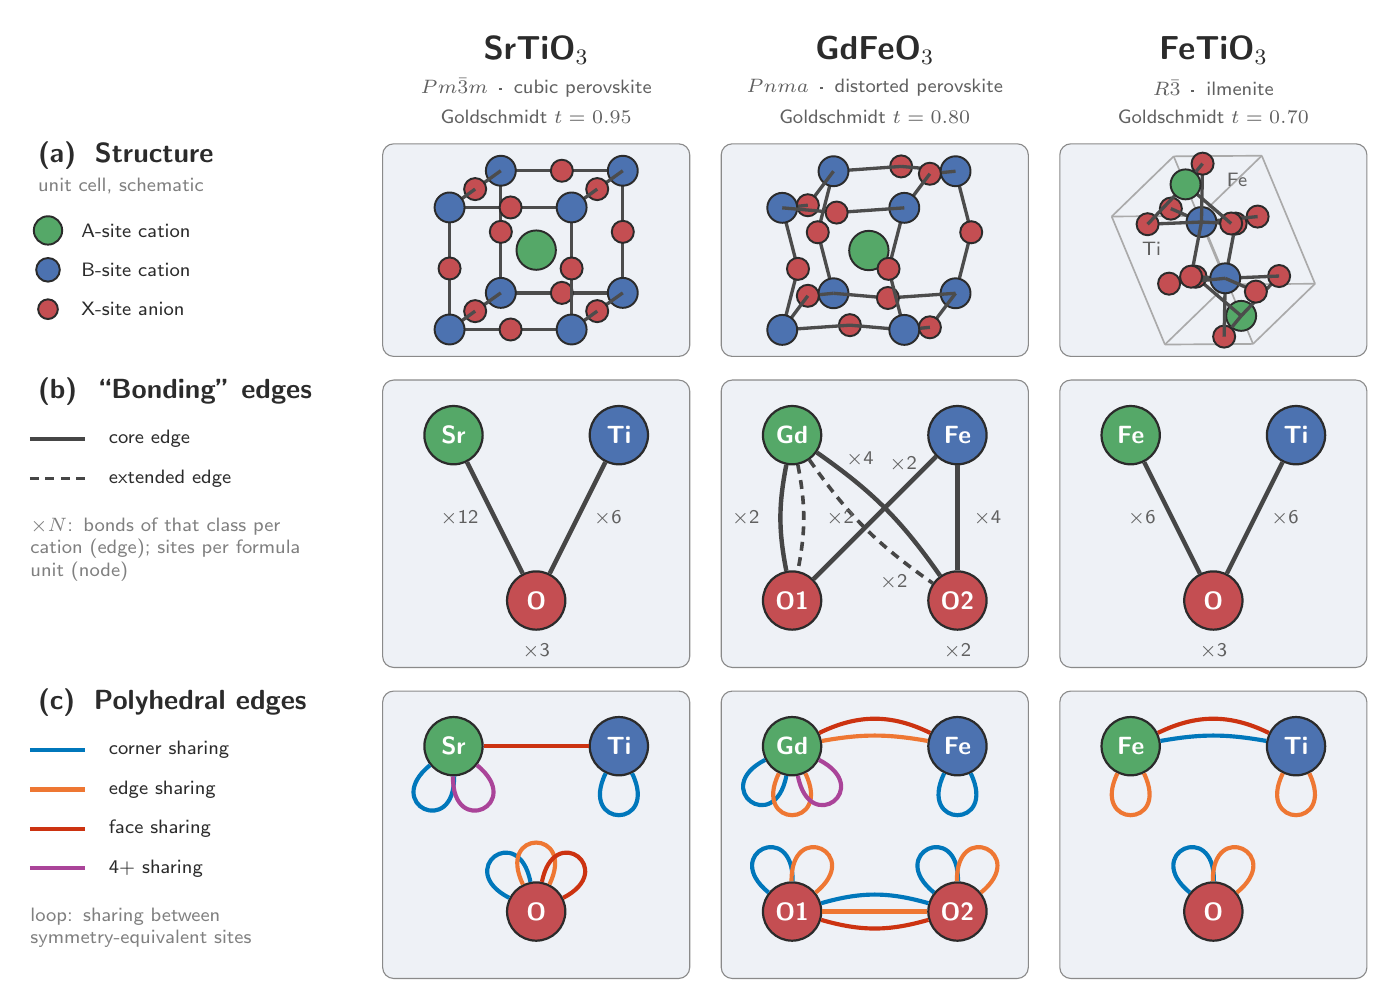
\begin{tikzpicture}

% =====================================================================
%  Geometry bookkeeping (cm)
%    legend column at x = -4.85 .. -0.7 ; material columns at
%    x0 = 0, 4.3, 8.6 ; panel x = x0-0.35 .. x0+3.55 (inner width 3.9)
%  Rows (absolute y):  header 10.55 / 10.91 / 11.38 ;
%    (a) motif    7.50 .. 10.20   (scope shift y = 7.65)
%    (b) bonding  3.55 ..  7.20   (scope shift y = 3.95)
%    (c) poly    -0.40 ..  3.25   (scope shift y = 0)
%  Row (b)/(c) graph panels share one node layout: cations top
%  (y = 2.55), anions bottom (y = 0.45), so the eye maps nodes across rows.
% =====================================================================

% ---------------------------------------------------------------------
%  Column headers
% ---------------------------------------------------------------------
\foreach \x/\formula/\proto/\tf in {%
    1.6/{SrTiO$_3$}/{$Pm\bar3m$ \,·\, cubic perovskite}/{0.95},
    5.9/{GdFeO$_3$}/{$Pnma$ \,·\, distorted perovskite}/{0.80},
    10.2/{FeTiO$_3$}/{$R\bar3$ \,·\, ilmenite}/{0.70}}{
  \node[ptitle, font=\large\bfseries\sffamily] at (\x,11.38) {\formula};
  \node[psub] at (\x,10.91) {\proto};
  \node[psub] at (\x,10.55) {Goldschmidt $t=\tf$};
}

% ---------------------------------------------------------------------
%  Row 1 — structure motifs (3-D ball-and-stick, oblique projection;
%  GENERATED by gen_motif3d.py (this directory) — edit that script, not this block)
% ---------------------------------------------------------------------
% SrTiO3: cubic cell, straight B-O-B cage, A at body centre
\begin{scope}[shift={(0,7.65)}]
  \draw[panelbox] (-0.35,-0.15) rectangle (3.55,2.55);
  \draw[mbond] (1.151,0.657) -- (1.926,0.657);
  \draw[mbond] (1.926,0.657) -- (2.700,0.657);
  \draw[mbond] (1.151,2.208) -- (1.926,2.208);
  \draw[mbond] (1.926,2.208) -- (2.700,2.208);
  \draw[mbond] (1.151,0.657) -- (1.151,1.432);
  \draw[mbond] (1.151,1.432) -- (1.151,2.208);
  \draw[mbond] (2.700,0.657) -- (2.700,1.432);
  \draw[mbond] (2.700,1.432) -- (2.700,2.208);
  \node[matomO] at (1.926,0.657) {};
  \node[matomO] at (1.926,2.208) {};
  \node[matomO] at (1.151,1.432) {};
  \node[matomO] at (2.700,1.432) {};
  \node[matomB] at (1.151,0.657) {};
  \node[matomB] at (1.151,2.208) {};
  \node[matomB] at (2.700,0.657) {};
  \node[matomB] at (2.700,2.208) {};
  \draw[mbond] (0.825,0.425) -- (1.151,0.657);
  \draw[mbond] (2.375,0.425) -- (2.700,0.657);
  \draw[mbond] (0.825,1.975) -- (1.151,2.208);
  \draw[mbond] (2.375,1.975) -- (2.700,2.208);
  \node[matomO] at (0.825,0.425) {};
  \node[matomO] at (2.375,0.425) {};
  \node[matomO] at (0.825,1.975) {};
  \node[matomO] at (2.375,1.975) {};
  \node[matomA] at (1.600,1.200) {};
  \draw[mbond] (0.500,0.192) -- (0.825,0.425);
  \draw[mbond] (2.050,0.192) -- (2.375,0.425);
  \draw[mbond] (0.500,1.742) -- (0.825,1.975);
  \draw[mbond] (2.050,1.742) -- (2.375,1.975);
  \draw[mbond] (0.500,0.192) -- (1.275,0.192);
  \draw[mbond] (1.275,0.192) -- (2.050,0.192);
  \draw[mbond] (0.500,1.742) -- (1.275,1.742);
  \draw[mbond] (1.275,1.742) -- (2.050,1.742);
  \draw[mbond] (0.500,0.192) -- (0.500,0.967);
  \draw[mbond] (0.500,0.967) -- (0.500,1.742);
  \draw[mbond] (2.050,0.192) -- (2.050,0.967);
  \draw[mbond] (2.050,0.967) -- (2.050,1.742);
  \node[matomO] at (1.275,0.192) {};
  \node[matomO] at (1.275,1.742) {};
  \node[matomO] at (0.500,0.967) {};
  \node[matomO] at (2.050,0.967) {};
  \node[matomB] at (0.500,0.192) {};
  \node[matomB] at (0.500,1.742) {};
  \node[matomB] at (2.050,0.192) {};
  \node[matomB] at (2.050,1.742) {};
\end{scope}
% GdFeO3: edge O tangentially displaced (octahedral tilt)
\begin{scope}[shift={(4.3,7.65)}]
  \draw[panelbox] (-0.35,-0.15) rectangle (3.55,2.55);
  \node[matomO] at (1.935,2.263) {};
  \draw[mbond] (1.076,2.202) -- (1.935,2.263);
  \draw[mbond] (1.935,2.263) -- (2.626,2.202);
  \draw[mbond] (1.076,0.652) -- (0.876,1.427);
  \draw[mbond] (0.876,1.427) -- (1.076,2.202);
  \draw[mbond] (2.626,0.652) -- (2.825,1.427);
  \draw[mbond] (2.825,1.427) -- (2.626,2.202);
  \node[matomO] at (0.876,1.427) {};
  \node[matomO] at (2.825,1.427) {};
  \node[matomB] at (1.076,0.652) {};
  \node[matomB] at (1.076,2.202) {};
  \node[matomB] at (2.626,0.652) {};
  \node[matomB] at (2.626,2.202) {};
  \draw[mbond] (1.076,0.652) -- (1.767,0.592);
  \draw[mbond] (1.767,0.592) -- (2.626,0.652);
  \node[matomO] at (1.767,0.592) {};
  \draw[mbond] (0.750,0.620) -- (1.076,0.652);
  \draw[mbond] (2.300,0.220) -- (2.626,0.652);
  \draw[mbond] (0.750,1.770) -- (1.076,2.202);
  \draw[mbond] (2.300,2.170) -- (2.626,2.202);
  \node[matomO] at (0.750,0.620) {};
  \node[matomO] at (2.300,0.220) {};
  \node[matomO] at (0.750,1.770) {};
  \node[matomO] at (2.300,2.170) {};
  \node[matomA] at (1.525,1.195) {};
  \draw[mbond] (0.425,0.187) -- (0.750,0.620);
  \draw[mbond] (1.975,0.187) -- (2.300,0.220);
  \draw[mbond] (0.425,1.737) -- (0.750,1.770);
  \draw[mbond] (1.975,1.737) -- (2.300,2.170);
  \node[matomO] at (1.284,0.247) {};
  \draw[mbond] (0.425,0.187) -- (1.284,0.247);
  \draw[mbond] (1.284,0.247) -- (1.975,0.187);
  \draw[mbond] (0.425,0.187) -- (0.625,0.962);
  \draw[mbond] (0.625,0.962) -- (0.425,1.737);
  \draw[mbond] (1.975,0.187) -- (1.775,0.962);
  \draw[mbond] (1.775,0.962) -- (1.975,1.737);
  \node[matomO] at (0.625,0.962) {};
  \node[matomO] at (1.775,0.962) {};
  \node[matomB] at (0.425,0.187) {};
  \node[matomB] at (0.425,1.737) {};
  \node[matomB] at (1.975,0.187) {};
  \node[matomB] at (1.975,1.737) {};
  \draw[mbond] (0.425,1.737) -- (1.116,1.677);
  \draw[mbond] (1.116,1.677) -- (1.975,1.737);
  \node[matomO] at (1.116,1.677) {};
\end{scope}
% FeTiO3: primitive rhombohedral cell, oblique view (orientation
% sweep option Q): the two face-sharing Fe-Ti pairs along the body
% diagonal with the shared O3 triangles shown in depth
\begin{scope}[shift={(8.6,7.65)}]
  \draw[panelbox] (-0.35,-0.15) rectangle (3.55,2.55);
  \draw[medge] (2.104,0.009) -- (2.891,0.773);
  \draw[medge] (2.104,0.009) -- (0.985,0.001);
  \draw[medge] (2.104,0.009) -- (1.427,1.635);
  \draw[medge] (2.891,0.773) -- (1.773,0.765);
  \draw[medge] (2.891,0.773) -- (2.215,2.399);
  \draw[medge] (0.985,0.001) -- (1.773,0.765);
  \draw[medge] (0.985,0.001) -- (0.309,1.627);
  \draw[medge] (1.427,1.635) -- (2.215,2.399);
  \draw[medge] (1.427,1.635) -- (0.309,1.627);
  \draw[medge] (1.773,0.765) -- (1.096,2.391);
  \draw[medge] (2.215,2.399) -- (1.096,2.391);
  \draw[medge] (0.309,1.627) -- (1.096,2.391);
  \node[matomA, minimum size=3.8mm] at (1.953,0.365) {};
  \draw[mbond] (1.953,0.365) -- (2.435,0.871);
  \node[matomO] at (2.435,0.871) {};
  \draw[mbond] (1.953,0.365) -- (1.374,0.862);
  \node[matomO] at (1.374,0.862) {};
  \draw[mbond] (1.953,0.365) -- (1.737,0.102);
  \draw[mbond] (1.751,0.842) -- (2.435,0.871);
  \draw[mbond] (1.751,0.842) -- (1.374,0.862);
  \node[matomO] at (1.883,1.537) {};
  \draw[mbond] (1.751,0.842) -- (1.883,1.537);
  \node[matomO] at (1.737,0.102) {};
  \draw[mbond] (1.751,0.842) -- (1.737,0.102);
  \node[matomB] at (1.751,0.842) {};
  \draw[mbond] (1.751,0.842) -- (2.140,0.673);
  \draw[mbond] (1.751,0.842) -- (1.038,0.774);
  \node[matomO] at (2.140,0.673) {};
  \node[matomO] at (1.038,0.774) {};
  \node[matomO] at (2.162,1.626) {};
  \node[matomO] at (1.060,1.727) {};
  \draw[mbond] (1.449,1.557) -- (2.162,1.626);
  \draw[mbond] (1.449,1.557) -- (1.060,1.727);
  \node[matomB] at (1.449,1.557) {};
  \draw[mbond] (1.449,1.557) -- (1.463,2.298);
  \node[matomO] at (1.463,2.298) {};
  \draw[mbond] (1.449,1.557) -- (1.317,0.863);
  \node[matomO] at (1.317,0.863) {};
  \draw[mbond] (1.449,1.557) -- (1.826,1.538);
  \draw[mbond] (1.449,1.557) -- (0.765,1.529);
  \draw[mbond] (1.247,2.035) -- (1.463,2.298);
  \node[matomO] at (1.826,1.538) {};
  \draw[mbond] (1.247,2.035) -- (1.826,1.538);
  \node[matomO] at (0.765,1.529) {};
  \draw[mbond] (1.247,2.035) -- (0.765,1.529);
  \node[matomA, minimum size=3.8mm] at (1.247,2.035) {};
  \node[psub, anchor=west] at (-0.457+2.104,2.086+0.009) {Fe};
  \node[psub, anchor=east] at (-1.045+2.104,1.208+0.009) {Ti};
\end{scope}

% ---------------------------------------------------------------------
%  Row 2 — bonding edges (condensed graphs)
%  node layout: cations top, anions bottom (identical in row 3)
% ---------------------------------------------------------------------
% ---- SrTiO3 : Sr-O core, Ti-O core ----------------------------------
\begin{scope}[shift={(0,3.95)}]
  \draw[panelbox] (-0.35,-0.40) rectangle (3.55,3.25);
  \node[siteA] (Sr) at (0.55,2.55) {Sr};
  \node[siteB] (Ti) at (2.65,2.55) {Ti};
  \node[siteO] (O)  at (1.60,0.45) {O};
  \draw[core] (Sr) -- (O);
  \draw[core] (Ti) -- (O);
  % bond multiplicities (bonds of this class per cation; builder mp-5229)
  \node[psub, anchor=east] at (0.99,1.50) {$\times$12};
  \node[psub, anchor=west] at (2.21,1.50) {$\times$6};
  % site multiplicity: 3 equivalent O per formula unit
  \node[psub, anchor=north] at (1.60,0.02) {$\times$3};
\end{scope}
% ---- GdFeO3 : Fe-O1, Fe-O2 core ; Gd-O1, Gd-O2 core+extended --------
\begin{scope}[shift={(4.3,3.95)}]
  \draw[panelbox] (-0.35,-0.40) rectangle (3.55,3.25);
  \node[siteA] (Gd) at (0.55,2.55) {Gd};
  \node[siteB] (Fe) at (2.65,2.55) {Fe};
  \node[siteO] (Oa) at (0.55,0.45) {O1};
  \node[siteO] (Ob) at (2.65,0.45) {O2};
  \draw[core] (Gd) to[bend right=11] (Oa);
  \draw[ext]  (Gd) to[bend left=11]  (Oa);
  \draw[core] (Gd) to[bend left=10]  (Ob);
  \draw[ext]  (Gd) to[bend right=10] (Ob);
  \draw[core] (Fe) -- (Oa);
  \draw[core] (Fe) -- (Ob);
  % bond multiplicities (bonds of this class per cation; builder mp-600576:
  % O1 = apical 4c, O2 = equatorial 8d; Gd core 2+4, ext 2+2; Fe 2+4)
  \node[psub, anchor=east]  at (0.26,1.50) {$\times$2};  % Gd-O1 core (left bulge)
  \node[psub, anchor=west]  at (0.86,1.50) {$\times$2};  % Gd-O1 ext (right bulge)
  \node[psub, anchor=south] at (1.41,2.02) {$\times$4};  % Gd-O2 core (upper bulge)
  \node[psub, anchor=north] at (1.84,0.90) {$\times$2};  % Gd-O2 ext (lower bulge)
  \node[psub, anchor=east]  at (2.26,2.18) {$\times$2};  % Fe-O1 (near Fe end)
  \node[psub, anchor=west]  at (2.73,1.50) {$\times$4};  % Fe-O2
  % site multiplicity: O2 = 8d, 2 sites per formula unit (O1 = 4c, 1)
  \node[psub, anchor=north] at (2.65,0.02) {$\times$2};
\end{scope}
% ---- FeTiO3 : Fe-O core, Ti-O core ----------------------------------
\begin{scope}[shift={(8.6,3.95)}]
  \draw[panelbox] (-0.35,-0.40) rectangle (3.55,3.25);
  \node[siteA] (Fe) at (0.55,2.55) {Fe};
  \node[siteB] (Ti) at (2.65,2.55) {Ti};
  \node[siteO] (O)  at (1.60,0.45) {O};
  \draw[core] (Fe) -- (O);
  \draw[core] (Ti) -- (O);
  % bond multiplicities (bonds of this class per cation; builder mp-19417)
  \node[psub, anchor=east] at (0.99,1.50) {$\times$6};
  \node[psub, anchor=west] at (2.21,1.50) {$\times$6};
  % site multiplicity: 3 equivalent O per formula unit
  \node[psub, anchor=north] at (1.60,0.02) {$\times$3};
\end{scope}

% ---------------------------------------------------------------------
%  Row 3 — polyhedral edges (condensed graphs, same node layout)
% ---------------------------------------------------------------------
% ---- SrTiO3 ---------------------------------------------------------
\begin{scope}[shift={(0,0)}]
  \draw[panelbox] (-0.35,-0.40) rectangle (3.55,3.25);
  \node[siteA] (Sr) at (0.55,2.55) {Sr};
  \node[siteB] (Ti) at (2.65,2.55) {Ti};
  \node[siteO] (O)  at (1.60,0.45) {O};
  \draw[pface] (Sr) -- (Ti);
  \gcloop{pcorner}{Sr}{245}
  \gcloop{pmulti}{Sr}{295}
  \gcloop{pcorner}{Ti}{270}
  \gcloop{pcorner}{O}{127}
  \gcloop{pedge}{O}{90}
  \gcloop{pface}{O}{53}
\end{scope}
% ---- GdFeO3 ---------------------------------------------------------
\begin{scope}[shift={(4.3,0)}]
  \draw[panelbox] (-0.35,-0.40) rectangle (3.55,3.25);
  \node[siteA] (Gd) at (0.55,2.55) {Gd};
  \node[siteB] (Fe) at (2.65,2.55) {Fe};
  \node[siteO] (Oa) at (0.55,0.45) {O1};
  \node[siteO] (Ob) at (2.65,0.45) {O2};
  \draw[pedge] (Gd) to[bend left=10] (Fe);
  \draw[pface] (Gd) to[bend left=26] (Fe);
  \draw[pcorner] (Oa) to[bend left=16] (Ob);
  \draw[pedge]   (Oa) -- (Ob);
  \draw[pface]   (Oa) to[bend right=16]  (Ob);
  \gcloop{pcorner}{Gd}{233}
  \gcloop{pedge}{Gd}{270}
  \gcloop{pmulti}{Gd}{307}
  \gcloop{pcorner}{Fe}{270}
  \gcloop{pcorner}{Oa}{115}
  \gcloop{pedge}{Oa}{65}
  \gcloop{pcorner}{Ob}{115}
  \gcloop{pedge}{Ob}{65}
\end{scope}
% ---- FeTiO3 ---------------------------------------------------------
\begin{scope}[shift={(8.6,0)}]
  \draw[panelbox] (-0.35,-0.40) rectangle (3.55,3.25);
  \node[siteA] (Fe) at (0.55,2.55) {Fe};
  \node[siteB] (Ti) at (2.65,2.55) {Ti};
  \node[siteO] (O)  at (1.60,0.45) {O};
  \draw[pcorner] (Fe) to[bend left=10] (Ti);
  \draw[pface]   (Fe) to[bend left=26] (Ti);
  \gcloop{pedge}{Fe}{270}
  \gcloop{pedge}{Ti}{270}
  \gcloop{pcorner}{O}{115}
  \gcloop{pedge}{O}{65}
\end{scope}

% ---------------------------------------------------------------------
%  Legend column (x ~ -4.85 .. -0.7): row tags (a)/(b)/(c) + keys.
%  Definitions (condensation rule, x N notation) live in the caption.
% ---------------------------------------------------------------------
\begin{scope}[shift={(-4.85,0)}]
  % ---- (a) structure ----
  \node[rowlbl] at (0,10.05) {(a)\; Structure};
  \node[rowlbl, text=ink!60, font=\scriptsize\sffamily] at (0,9.67) {unit cell, schematic};
  \node[matomA, minimum size=3.6mm] at (0.25,9.10) {}; \node[leglbl] at (0.55,9.10) {A-site cation};
  \node[matomB, minimum size=3.0mm] at (0.25,8.60) {}; \node[leglbl] at (0.55,8.60) {B-site cation};
  \node[matomO, minimum size=2.5mm] at (0.25,8.10) {}; \node[leglbl] at (0.55,8.10) {X-site anion};

  % ---- (b) bonding edges ----
  \node[rowlbl] at (0,7.05) {(b)\; ``Bonding'' edges};
  \draw[core] (0.02,6.45) -- (0.72,6.45); \node[leglbl] at (0.90,6.45) {core edge};
  \draw[ext]  (0.02,5.95) -- (0.72,5.95); \node[leglbl] at (0.90,5.95) {extended edge};
  \node[leghint] at (0.02,5.45)
    {$\times N$: bonds of that class per cation (edge); sites per formula unit (node)};

  % ---- (c) polyhedral edges ----
  \node[rowlbl] at (0,3.10) {(c)\; Polyhedral edges};
  \draw[pcorner] (0.02,2.50) -- (0.72,2.50); \node[leglbl] at (0.90,2.50) {corner sharing};
  \draw[pedge]   (0.02,2.00) -- (0.72,2.00); \node[leglbl] at (0.90,2.00) {edge sharing};
  \draw[pface]   (0.02,1.50) -- (0.72,1.50); \node[leglbl] at (0.90,1.50) {face sharing};
  \draw[pmulti]  (0.02,1.00) -- (0.72,1.00); \node[leglbl] at (0.90,1.00) {4+ sharing};
  \node[leghint] at (0.02,0.50)
    {loop: sharing between symmetry-equivalent sites};
\end{scope}

\end{tikzpicture}
\endgroup
}
%       \caption{Condensed crystal graphs of three $ABO_3$ compounds:
%         cubic perovskite SrTiO$_3$ (mp-5229), orthorhombically
%         distorted perovskite GdFeO$_3$ (mp-600576) and ilmenite
%         FeTiO$_3$ (mp-19417); $t$ is the Goldschmidt tolerance factor.
%         (a)~Schematic unit cells.  (b)~Bonding edges and
%         (c)~polyhedral edges of the crystal graph, condensed by
%         symmetry: one node per symmetry-inequivalent site and one
%         drawn edge per symmetry class of edges; loops denote sharing
%         between symmetry-equivalent sites.  $\times N$ on an edge is
%         the number of bonds of that class per cation, $\times N$ under
%         a node the number of such sites per formula unit.  All three
%         graphs share the $B$--O core bonding motif, and the distortion
%         of GdFeO$_3$ appears as split core/extended Gd--O bond classes.
%         Polyhedral edges separate the structure types: both
%         perovskites carry the $B$--$B$ corner-sharing loop, whereas
%         ilmenite has no like-cation corner sharing -- its cations form
%         edge-sharing layers linked by Fe--Ti face sharing.}
%       \label{fig:graph-construction}
%     \end{figure*}
%
%  Content: all graph content is EXTRACTED from the real v4 builder
%  output (build_crystal_graph_from_structure on MP structures mp-5229 /
%  mp-600576 / mp-19417, node orbits by SpacegroupAnalyzer) — one node
%  per symmetry-inequivalent site, one drawn edge per symmetry class.
%  Layout: 3x3 grid, materials as columns, rows (top -> bottom)
%    (a) structure motif (3-D ball-and-stick cells; GENERATED by
%        gen_motif3d.py — edit that script, not the Row-1 block)
%    (b) bonding edges   (core solid / extended dashed)
%    (c) polyhedral edges (corner / edge / face / 4+ sharing)
%  Story: both perovskites share the B-B corner-sharing loop; ilmenite
%  has NO like-cation corner sharing (edge loops + Fe-Ti face sharing).
%  Native size ~17.4 x 11.7 cm (aspect 1.5) so that at \textwidth of a
%  two-column page the \scriptsize labels stay ~7 pt.
%  Palette/styles match gps_encoder_fig.tex.
% =====================================================================
\begingroup

% ---- palette (shared with gps_encoder_fig.tex) ----------------------
\definecolor{Bcol}{HTML}{4C72B0}    % B-site / metal cation
\definecolor{Ocol}{HTML}{C44E52}    % anion (oxygen)
\definecolor{Acol}{HTML}{55A868}    % A-site large cation
\definecolor{panel}{HTML}{EEF1F6}   % light panel fill
\definecolor{ink}{HTML}{2B2B2B}
% polyhedral-edge classes (colorblind-safe, echoes the old blue/orange/red/purple)
\definecolor{cCorner}{HTML}{0077BB}
\definecolor{cEdge}{HTML}{EE7733}
\definecolor{cFace}{HTML}{CC3311}
\definecolor{cMulti}{HTML}{AA4499}

% ---- shared styles (local to this group) ----------------------------
\tikzset{
  siteA/.style={circle, draw=ink, thick, fill=Acol, minimum size=7.4mm,
                inner sep=0pt, font=\small\bfseries\sffamily, text=white},
  siteB/.style={circle, draw=ink, thick, fill=Bcol, minimum size=7.4mm,
                inner sep=0pt, font=\small\bfseries\sffamily, text=white},
  siteO/.style={circle, draw=ink, thick, fill=Ocol, minimum size=7.4mm,
                inner sep=0pt, font=\small\bfseries\sffamily, text=white},
  core/.style={line width=1.6pt, gray!55!black},
  ext/.style={line width=1.3pt, gray!55!black, dash pattern=on 3.2pt off 2.4pt},
  pcorner/.style={line width=1.5pt, cCorner},
  pedge/.style={line width=1.5pt, cEdge},
  pface/.style={line width=1.5pt, cFace},
  pmulti/.style={line width=1.5pt, cMulti},
  panelbox/.style={draw=ink!55, rounded corners=4pt, fill=panel},
  ptitle/.style={font=\bfseries\sffamily, text=ink},
  psub/.style={font=\scriptsize\sffamily, text=ink!75},
  rowlbl/.style={font=\bfseries\sffamily, text=ink, anchor=west},
  leglbl/.style={font=\scriptsize\sffamily, text=ink, anchor=west},
  leghint/.style={font=\scriptsize\sffamily, text=ink!60, anchor=north west,
                  text width=36mm, align=left, inner sep=0pt},
  % motif ingredients (ball-and-stick, matching the gps_encoder structure panel;
  % sizes keep gps_encoder's atom/spacing ratio at this row's 1.0 grid spacing)
  matomA/.style={circle, draw=ink, line width=0.7pt, fill=Acol, minimum size=5.0mm, inner sep=0pt},
  matomB/.style={circle, draw=ink, line width=0.7pt, fill=Bcol, minimum size=3.8mm, inner sep=0pt},
  matomO/.style={circle, draw=ink, line width=0.7pt, fill=Ocol, minimum size=2.8mm, inner sep=0pt},
  mbond/.style={line width=1.2pt, gray!60!black},
  medge/.style={line width=0.6pt, ink!40},
}

% loop macro: \gcloop{style}{node}{center direction in deg}
% \providecommand (not \newcommand): inert if the main doc, or a second
% \input of this fragment, already defined it.
\providecommand{\gcloop}[3]{%
  \path[#1] (#2) edge[out=#3+26, in=#3-26, looseness=6, min distance=6mm] (#2);}

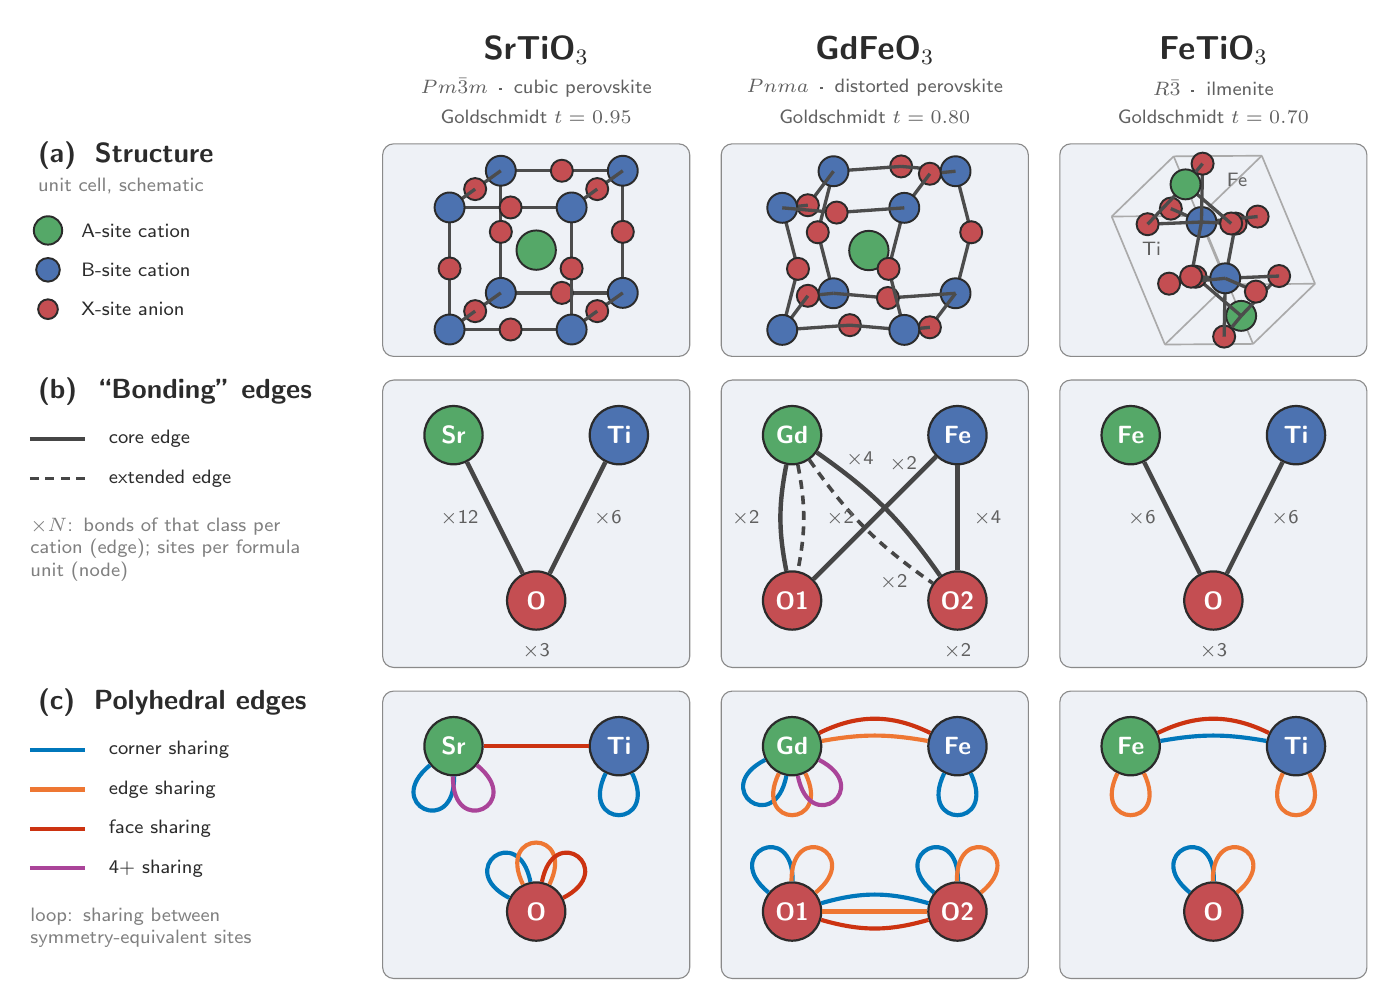
\begin{tikzpicture}

% =====================================================================
%  Geometry bookkeeping (cm)
%    legend column at x = -4.85 .. -0.7 ; material columns at
%    x0 = 0, 4.3, 8.6 ; panel x = x0-0.35 .. x0+3.55 (inner width 3.9)
%  Rows (absolute y):  header 10.55 / 10.91 / 11.38 ;
%    (a) motif    7.50 .. 10.20   (scope shift y = 7.65)
%    (b) bonding  3.55 ..  7.20   (scope shift y = 3.95)
%    (c) poly    -0.40 ..  3.25   (scope shift y = 0)
%  Row (b)/(c) graph panels share one node layout: cations top
%  (y = 2.55), anions bottom (y = 0.45), so the eye maps nodes across rows.
% =====================================================================

% ---------------------------------------------------------------------
%  Column headers
% ---------------------------------------------------------------------
\foreach \x/\formula/\proto/\tf in {%
    1.6/{SrTiO$_3$}/{$Pm\bar3m$ \,·\, cubic perovskite}/{0.95},
    5.9/{GdFeO$_3$}/{$Pnma$ \,·\, distorted perovskite}/{0.80},
    10.2/{FeTiO$_3$}/{$R\bar3$ \,·\, ilmenite}/{0.70}}{
  \node[ptitle, font=\large\bfseries\sffamily] at (\x,11.38) {\formula};
  \node[psub] at (\x,10.91) {\proto};
  \node[psub] at (\x,10.55) {Goldschmidt $t=\tf$};
}

% ---------------------------------------------------------------------
%  Row 1 — structure motifs (3-D ball-and-stick, oblique projection;
%  GENERATED by gen_motif3d.py (this directory) — edit that script, not this block)
% ---------------------------------------------------------------------
% SrTiO3: cubic cell, straight B-O-B cage, A at body centre
\begin{scope}[shift={(0,7.65)}]
  \draw[panelbox] (-0.35,-0.15) rectangle (3.55,2.55);
  \draw[mbond] (1.151,0.657) -- (1.926,0.657);
  \draw[mbond] (1.926,0.657) -- (2.700,0.657);
  \draw[mbond] (1.151,2.208) -- (1.926,2.208);
  \draw[mbond] (1.926,2.208) -- (2.700,2.208);
  \draw[mbond] (1.151,0.657) -- (1.151,1.432);
  \draw[mbond] (1.151,1.432) -- (1.151,2.208);
  \draw[mbond] (2.700,0.657) -- (2.700,1.432);
  \draw[mbond] (2.700,1.432) -- (2.700,2.208);
  \node[matomO] at (1.926,0.657) {};
  \node[matomO] at (1.926,2.208) {};
  \node[matomO] at (1.151,1.432) {};
  \node[matomO] at (2.700,1.432) {};
  \node[matomB] at (1.151,0.657) {};
  \node[matomB] at (1.151,2.208) {};
  \node[matomB] at (2.700,0.657) {};
  \node[matomB] at (2.700,2.208) {};
  \draw[mbond] (0.825,0.425) -- (1.151,0.657);
  \draw[mbond] (2.375,0.425) -- (2.700,0.657);
  \draw[mbond] (0.825,1.975) -- (1.151,2.208);
  \draw[mbond] (2.375,1.975) -- (2.700,2.208);
  \node[matomO] at (0.825,0.425) {};
  \node[matomO] at (2.375,0.425) {};
  \node[matomO] at (0.825,1.975) {};
  \node[matomO] at (2.375,1.975) {};
  \node[matomA] at (1.600,1.200) {};
  \draw[mbond] (0.500,0.192) -- (0.825,0.425);
  \draw[mbond] (2.050,0.192) -- (2.375,0.425);
  \draw[mbond] (0.500,1.742) -- (0.825,1.975);
  \draw[mbond] (2.050,1.742) -- (2.375,1.975);
  \draw[mbond] (0.500,0.192) -- (1.275,0.192);
  \draw[mbond] (1.275,0.192) -- (2.050,0.192);
  \draw[mbond] (0.500,1.742) -- (1.275,1.742);
  \draw[mbond] (1.275,1.742) -- (2.050,1.742);
  \draw[mbond] (0.500,0.192) -- (0.500,0.967);
  \draw[mbond] (0.500,0.967) -- (0.500,1.742);
  \draw[mbond] (2.050,0.192) -- (2.050,0.967);
  \draw[mbond] (2.050,0.967) -- (2.050,1.742);
  \node[matomO] at (1.275,0.192) {};
  \node[matomO] at (1.275,1.742) {};
  \node[matomO] at (0.500,0.967) {};
  \node[matomO] at (2.050,0.967) {};
  \node[matomB] at (0.500,0.192) {};
  \node[matomB] at (0.500,1.742) {};
  \node[matomB] at (2.050,0.192) {};
  \node[matomB] at (2.050,1.742) {};
\end{scope}
% GdFeO3: edge O tangentially displaced (octahedral tilt)
\begin{scope}[shift={(4.3,7.65)}]
  \draw[panelbox] (-0.35,-0.15) rectangle (3.55,2.55);
  \node[matomO] at (1.935,2.263) {};
  \draw[mbond] (1.076,2.202) -- (1.935,2.263);
  \draw[mbond] (1.935,2.263) -- (2.626,2.202);
  \draw[mbond] (1.076,0.652) -- (0.876,1.427);
  \draw[mbond] (0.876,1.427) -- (1.076,2.202);
  \draw[mbond] (2.626,0.652) -- (2.825,1.427);
  \draw[mbond] (2.825,1.427) -- (2.626,2.202);
  \node[matomO] at (0.876,1.427) {};
  \node[matomO] at (2.825,1.427) {};
  \node[matomB] at (1.076,0.652) {};
  \node[matomB] at (1.076,2.202) {};
  \node[matomB] at (2.626,0.652) {};
  \node[matomB] at (2.626,2.202) {};
  \draw[mbond] (1.076,0.652) -- (1.767,0.592);
  \draw[mbond] (1.767,0.592) -- (2.626,0.652);
  \node[matomO] at (1.767,0.592) {};
  \draw[mbond] (0.750,0.620) -- (1.076,0.652);
  \draw[mbond] (2.300,0.220) -- (2.626,0.652);
  \draw[mbond] (0.750,1.770) -- (1.076,2.202);
  \draw[mbond] (2.300,2.170) -- (2.626,2.202);
  \node[matomO] at (0.750,0.620) {};
  \node[matomO] at (2.300,0.220) {};
  \node[matomO] at (0.750,1.770) {};
  \node[matomO] at (2.300,2.170) {};
  \node[matomA] at (1.525,1.195) {};
  \draw[mbond] (0.425,0.187) -- (0.750,0.620);
  \draw[mbond] (1.975,0.187) -- (2.300,0.220);
  \draw[mbond] (0.425,1.737) -- (0.750,1.770);
  \draw[mbond] (1.975,1.737) -- (2.300,2.170);
  \node[matomO] at (1.284,0.247) {};
  \draw[mbond] (0.425,0.187) -- (1.284,0.247);
  \draw[mbond] (1.284,0.247) -- (1.975,0.187);
  \draw[mbond] (0.425,0.187) -- (0.625,0.962);
  \draw[mbond] (0.625,0.962) -- (0.425,1.737);
  \draw[mbond] (1.975,0.187) -- (1.775,0.962);
  \draw[mbond] (1.775,0.962) -- (1.975,1.737);
  \node[matomO] at (0.625,0.962) {};
  \node[matomO] at (1.775,0.962) {};
  \node[matomB] at (0.425,0.187) {};
  \node[matomB] at (0.425,1.737) {};
  \node[matomB] at (1.975,0.187) {};
  \node[matomB] at (1.975,1.737) {};
  \draw[mbond] (0.425,1.737) -- (1.116,1.677);
  \draw[mbond] (1.116,1.677) -- (1.975,1.737);
  \node[matomO] at (1.116,1.677) {};
\end{scope}
% FeTiO3: primitive rhombohedral cell, oblique view (orientation
% sweep option Q): the two face-sharing Fe-Ti pairs along the body
% diagonal with the shared O3 triangles shown in depth
\begin{scope}[shift={(8.6,7.65)}]
  \draw[panelbox] (-0.35,-0.15) rectangle (3.55,2.55);
  \draw[medge] (2.104,0.009) -- (2.891,0.773);
  \draw[medge] (2.104,0.009) -- (0.985,0.001);
  \draw[medge] (2.104,0.009) -- (1.427,1.635);
  \draw[medge] (2.891,0.773) -- (1.773,0.765);
  \draw[medge] (2.891,0.773) -- (2.215,2.399);
  \draw[medge] (0.985,0.001) -- (1.773,0.765);
  \draw[medge] (0.985,0.001) -- (0.309,1.627);
  \draw[medge] (1.427,1.635) -- (2.215,2.399);
  \draw[medge] (1.427,1.635) -- (0.309,1.627);
  \draw[medge] (1.773,0.765) -- (1.096,2.391);
  \draw[medge] (2.215,2.399) -- (1.096,2.391);
  \draw[medge] (0.309,1.627) -- (1.096,2.391);
  \node[matomA, minimum size=3.8mm] at (1.953,0.365) {};
  \draw[mbond] (1.953,0.365) -- (2.435,0.871);
  \node[matomO] at (2.435,0.871) {};
  \draw[mbond] (1.953,0.365) -- (1.374,0.862);
  \node[matomO] at (1.374,0.862) {};
  \draw[mbond] (1.953,0.365) -- (1.737,0.102);
  \draw[mbond] (1.751,0.842) -- (2.435,0.871);
  \draw[mbond] (1.751,0.842) -- (1.374,0.862);
  \node[matomO] at (1.883,1.537) {};
  \draw[mbond] (1.751,0.842) -- (1.883,1.537);
  \node[matomO] at (1.737,0.102) {};
  \draw[mbond] (1.751,0.842) -- (1.737,0.102);
  \node[matomB] at (1.751,0.842) {};
  \draw[mbond] (1.751,0.842) -- (2.140,0.673);
  \draw[mbond] (1.751,0.842) -- (1.038,0.774);
  \node[matomO] at (2.140,0.673) {};
  \node[matomO] at (1.038,0.774) {};
  \node[matomO] at (2.162,1.626) {};
  \node[matomO] at (1.060,1.727) {};
  \draw[mbond] (1.449,1.557) -- (2.162,1.626);
  \draw[mbond] (1.449,1.557) -- (1.060,1.727);
  \node[matomB] at (1.449,1.557) {};
  \draw[mbond] (1.449,1.557) -- (1.463,2.298);
  \node[matomO] at (1.463,2.298) {};
  \draw[mbond] (1.449,1.557) -- (1.317,0.863);
  \node[matomO] at (1.317,0.863) {};
  \draw[mbond] (1.449,1.557) -- (1.826,1.538);
  \draw[mbond] (1.449,1.557) -- (0.765,1.529);
  \draw[mbond] (1.247,2.035) -- (1.463,2.298);
  \node[matomO] at (1.826,1.538) {};
  \draw[mbond] (1.247,2.035) -- (1.826,1.538);
  \node[matomO] at (0.765,1.529) {};
  \draw[mbond] (1.247,2.035) -- (0.765,1.529);
  \node[matomA, minimum size=3.8mm] at (1.247,2.035) {};
  \node[psub, anchor=west] at (-0.457+2.104,2.086+0.009) {Fe};
  \node[psub, anchor=east] at (-1.045+2.104,1.208+0.009) {Ti};
\end{scope}

% ---------------------------------------------------------------------
%  Row 2 — bonding edges (condensed graphs)
%  node layout: cations top, anions bottom (identical in row 3)
% ---------------------------------------------------------------------
% ---- SrTiO3 : Sr-O core, Ti-O core ----------------------------------
\begin{scope}[shift={(0,3.95)}]
  \draw[panelbox] (-0.35,-0.40) rectangle (3.55,3.25);
  \node[siteA] (Sr) at (0.55,2.55) {Sr};
  \node[siteB] (Ti) at (2.65,2.55) {Ti};
  \node[siteO] (O)  at (1.60,0.45) {O};
  \draw[core] (Sr) -- (O);
  \draw[core] (Ti) -- (O);
  % bond multiplicities (bonds of this class per cation; builder mp-5229)
  \node[psub, anchor=east] at (0.99,1.50) {$\times$12};
  \node[psub, anchor=west] at (2.21,1.50) {$\times$6};
  % site multiplicity: 3 equivalent O per formula unit
  \node[psub, anchor=north] at (1.60,0.02) {$\times$3};
\end{scope}
% ---- GdFeO3 : Fe-O1, Fe-O2 core ; Gd-O1, Gd-O2 core+extended --------
\begin{scope}[shift={(4.3,3.95)}]
  \draw[panelbox] (-0.35,-0.40) rectangle (3.55,3.25);
  \node[siteA] (Gd) at (0.55,2.55) {Gd};
  \node[siteB] (Fe) at (2.65,2.55) {Fe};
  \node[siteO] (Oa) at (0.55,0.45) {O1};
  \node[siteO] (Ob) at (2.65,0.45) {O2};
  \draw[core] (Gd) to[bend right=11] (Oa);
  \draw[ext]  (Gd) to[bend left=11]  (Oa);
  \draw[core] (Gd) to[bend left=10]  (Ob);
  \draw[ext]  (Gd) to[bend right=10] (Ob);
  \draw[core] (Fe) -- (Oa);
  \draw[core] (Fe) -- (Ob);
  % bond multiplicities (bonds of this class per cation; builder mp-600576:
  % O1 = apical 4c, O2 = equatorial 8d; Gd core 2+4, ext 2+2; Fe 2+4)
  \node[psub, anchor=east]  at (0.26,1.50) {$\times$2};  % Gd-O1 core (left bulge)
  \node[psub, anchor=west]  at (0.86,1.50) {$\times$2};  % Gd-O1 ext (right bulge)
  \node[psub, anchor=south] at (1.41,2.02) {$\times$4};  % Gd-O2 core (upper bulge)
  \node[psub, anchor=north] at (1.84,0.90) {$\times$2};  % Gd-O2 ext (lower bulge)
  \node[psub, anchor=east]  at (2.26,2.18) {$\times$2};  % Fe-O1 (near Fe end)
  \node[psub, anchor=west]  at (2.73,1.50) {$\times$4};  % Fe-O2
  % site multiplicity: O2 = 8d, 2 sites per formula unit (O1 = 4c, 1)
  \node[psub, anchor=north] at (2.65,0.02) {$\times$2};
\end{scope}
% ---- FeTiO3 : Fe-O core, Ti-O core ----------------------------------
\begin{scope}[shift={(8.6,3.95)}]
  \draw[panelbox] (-0.35,-0.40) rectangle (3.55,3.25);
  \node[siteA] (Fe) at (0.55,2.55) {Fe};
  \node[siteB] (Ti) at (2.65,2.55) {Ti};
  \node[siteO] (O)  at (1.60,0.45) {O};
  \draw[core] (Fe) -- (O);
  \draw[core] (Ti) -- (O);
  % bond multiplicities (bonds of this class per cation; builder mp-19417)
  \node[psub, anchor=east] at (0.99,1.50) {$\times$6};
  \node[psub, anchor=west] at (2.21,1.50) {$\times$6};
  % site multiplicity: 3 equivalent O per formula unit
  \node[psub, anchor=north] at (1.60,0.02) {$\times$3};
\end{scope}

% ---------------------------------------------------------------------
%  Row 3 — polyhedral edges (condensed graphs, same node layout)
% ---------------------------------------------------------------------
% ---- SrTiO3 ---------------------------------------------------------
\begin{scope}[shift={(0,0)}]
  \draw[panelbox] (-0.35,-0.40) rectangle (3.55,3.25);
  \node[siteA] (Sr) at (0.55,2.55) {Sr};
  \node[siteB] (Ti) at (2.65,2.55) {Ti};
  \node[siteO] (O)  at (1.60,0.45) {O};
  \draw[pface] (Sr) -- (Ti);
  \gcloop{pcorner}{Sr}{245}
  \gcloop{pmulti}{Sr}{295}
  \gcloop{pcorner}{Ti}{270}
  \gcloop{pcorner}{O}{127}
  \gcloop{pedge}{O}{90}
  \gcloop{pface}{O}{53}
\end{scope}
% ---- GdFeO3 ---------------------------------------------------------
\begin{scope}[shift={(4.3,0)}]
  \draw[panelbox] (-0.35,-0.40) rectangle (3.55,3.25);
  \node[siteA] (Gd) at (0.55,2.55) {Gd};
  \node[siteB] (Fe) at (2.65,2.55) {Fe};
  \node[siteO] (Oa) at (0.55,0.45) {O1};
  \node[siteO] (Ob) at (2.65,0.45) {O2};
  \draw[pedge] (Gd) to[bend left=10] (Fe);
  \draw[pface] (Gd) to[bend left=26] (Fe);
  \draw[pcorner] (Oa) to[bend left=16] (Ob);
  \draw[pedge]   (Oa) -- (Ob);
  \draw[pface]   (Oa) to[bend right=16]  (Ob);
  \gcloop{pcorner}{Gd}{233}
  \gcloop{pedge}{Gd}{270}
  \gcloop{pmulti}{Gd}{307}
  \gcloop{pcorner}{Fe}{270}
  \gcloop{pcorner}{Oa}{115}
  \gcloop{pedge}{Oa}{65}
  \gcloop{pcorner}{Ob}{115}
  \gcloop{pedge}{Ob}{65}
\end{scope}
% ---- FeTiO3 ---------------------------------------------------------
\begin{scope}[shift={(8.6,0)}]
  \draw[panelbox] (-0.35,-0.40) rectangle (3.55,3.25);
  \node[siteA] (Fe) at (0.55,2.55) {Fe};
  \node[siteB] (Ti) at (2.65,2.55) {Ti};
  \node[siteO] (O)  at (1.60,0.45) {O};
  \draw[pcorner] (Fe) to[bend left=10] (Ti);
  \draw[pface]   (Fe) to[bend left=26] (Ti);
  \gcloop{pedge}{Fe}{270}
  \gcloop{pedge}{Ti}{270}
  \gcloop{pcorner}{O}{115}
  \gcloop{pedge}{O}{65}
\end{scope}

% ---------------------------------------------------------------------
%  Legend column (x ~ -4.85 .. -0.7): row tags (a)/(b)/(c) + keys.
%  Definitions (condensation rule, x N notation) live in the caption.
% ---------------------------------------------------------------------
\begin{scope}[shift={(-4.85,0)}]
  % ---- (a) structure ----
  \node[rowlbl] at (0,10.05) {(a)\; Structure};
  \node[rowlbl, text=ink!60, font=\scriptsize\sffamily] at (0,9.67) {unit cell, schematic};
  \node[matomA, minimum size=3.6mm] at (0.25,9.10) {}; \node[leglbl] at (0.55,9.10) {A-site cation};
  \node[matomB, minimum size=3.0mm] at (0.25,8.60) {}; \node[leglbl] at (0.55,8.60) {B-site cation};
  \node[matomO, minimum size=2.5mm] at (0.25,8.10) {}; \node[leglbl] at (0.55,8.10) {X-site anion};

  % ---- (b) bonding edges ----
  \node[rowlbl] at (0,7.05) {(b)\; ``Bonding'' edges};
  \draw[core] (0.02,6.45) -- (0.72,6.45); \node[leglbl] at (0.90,6.45) {core edge};
  \draw[ext]  (0.02,5.95) -- (0.72,5.95); \node[leglbl] at (0.90,5.95) {extended edge};
  \node[leghint] at (0.02,5.45)
    {$\times N$: bonds of that class per cation (edge); sites per formula unit (node)};

  % ---- (c) polyhedral edges ----
  \node[rowlbl] at (0,3.10) {(c)\; Polyhedral edges};
  \draw[pcorner] (0.02,2.50) -- (0.72,2.50); \node[leglbl] at (0.90,2.50) {corner sharing};
  \draw[pedge]   (0.02,2.00) -- (0.72,2.00); \node[leglbl] at (0.90,2.00) {edge sharing};
  \draw[pface]   (0.02,1.50) -- (0.72,1.50); \node[leglbl] at (0.90,1.50) {face sharing};
  \draw[pmulti]  (0.02,1.00) -- (0.72,1.00); \node[leglbl] at (0.90,1.00) {4+ sharing};
  \node[leghint] at (0.02,0.50)
    {loop: sharing between symmetry-equivalent sites};
\end{scope}

\end{tikzpicture}
\endgroup
}
%       \caption{Condensed crystal graphs of three $ABO_3$ compounds:
%         cubic perovskite SrTiO$_3$ (mp-5229), orthorhombically
%         distorted perovskite GdFeO$_3$ (mp-600576) and ilmenite
%         FeTiO$_3$ (mp-19417); $t$ is the Goldschmidt tolerance factor.
%         (a)~Schematic unit cells.  (b)~Bonding edges and
%         (c)~polyhedral edges of the crystal graph, condensed by
%         symmetry: one node per symmetry-inequivalent site and one
%         drawn edge per symmetry class of edges; loops denote sharing
%         between symmetry-equivalent sites.  $\times N$ on an edge is
%         the number of bonds of that class per cation, $\times N$ under
%         a node the number of such sites per formula unit.  All three
%         graphs share the $B$--O core bonding motif, and the distortion
%         of GdFeO$_3$ appears as split core/extended Gd--O bond classes.
%         Polyhedral edges separate the structure types: both
%         perovskites carry the $B$--$B$ corner-sharing loop, whereas
%         ilmenite has no like-cation corner sharing -- its cations form
%         edge-sharing layers linked by Fe--Ti face sharing.}
%       \label{fig:graph-construction}
%     \end{figure*}
%
%  Content: all graph content is EXTRACTED from the real v4 builder
%  output (build_crystal_graph_from_structure on MP structures mp-5229 /
%  mp-600576 / mp-19417, node orbits by SpacegroupAnalyzer) — one node
%  per symmetry-inequivalent site, one drawn edge per symmetry class.
%  Layout: 3x3 grid, materials as columns, rows (top -> bottom)
%    (a) structure motif (3-D ball-and-stick cells; GENERATED by
%        gen_motif3d.py — edit that script, not the Row-1 block)
%    (b) bonding edges   (core solid / extended dashed)
%    (c) polyhedral edges (corner / edge / face / 4+ sharing)
%  Story: both perovskites share the B-B corner-sharing loop; ilmenite
%  has NO like-cation corner sharing (edge loops + Fe-Ti face sharing).
%  Native size ~17.4 x 11.7 cm (aspect 1.5) so that at \textwidth of a
%  two-column page the \scriptsize labels stay ~7 pt.
%  Palette/styles match gps_encoder_fig.tex.
% =====================================================================
\begingroup

% ---- palette (shared with gps_encoder_fig.tex) ----------------------
\definecolor{Bcol}{HTML}{4C72B0}    % B-site / metal cation
\definecolor{Ocol}{HTML}{C44E52}    % anion (oxygen)
\definecolor{Acol}{HTML}{55A868}    % A-site large cation
\definecolor{panel}{HTML}{EEF1F6}   % light panel fill
\definecolor{ink}{HTML}{2B2B2B}
% polyhedral-edge classes (colorblind-safe, echoes the old blue/orange/red/purple)
\definecolor{cCorner}{HTML}{0077BB}
\definecolor{cEdge}{HTML}{EE7733}
\definecolor{cFace}{HTML}{CC3311}
\definecolor{cMulti}{HTML}{AA4499}

% ---- shared styles (local to this group) ----------------------------
\tikzset{
  siteA/.style={circle, draw=ink, thick, fill=Acol, minimum size=7.4mm,
                inner sep=0pt, font=\small\bfseries\sffamily, text=white},
  siteB/.style={circle, draw=ink, thick, fill=Bcol, minimum size=7.4mm,
                inner sep=0pt, font=\small\bfseries\sffamily, text=white},
  siteO/.style={circle, draw=ink, thick, fill=Ocol, minimum size=7.4mm,
                inner sep=0pt, font=\small\bfseries\sffamily, text=white},
  core/.style={line width=1.6pt, gray!55!black},
  ext/.style={line width=1.3pt, gray!55!black, dash pattern=on 3.2pt off 2.4pt},
  pcorner/.style={line width=1.5pt, cCorner},
  pedge/.style={line width=1.5pt, cEdge},
  pface/.style={line width=1.5pt, cFace},
  pmulti/.style={line width=1.5pt, cMulti},
  panelbox/.style={draw=ink!55, rounded corners=4pt, fill=panel},
  ptitle/.style={font=\bfseries\sffamily, text=ink},
  psub/.style={font=\scriptsize\sffamily, text=ink!75},
  rowlbl/.style={font=\bfseries\sffamily, text=ink, anchor=west},
  leglbl/.style={font=\scriptsize\sffamily, text=ink, anchor=west},
  leghint/.style={font=\scriptsize\sffamily, text=ink!60, anchor=north west,
                  text width=36mm, align=left, inner sep=0pt},
  % motif ingredients (ball-and-stick, matching the gps_encoder structure panel;
  % sizes keep gps_encoder's atom/spacing ratio at this row's 1.0 grid spacing)
  matomA/.style={circle, draw=ink, line width=0.7pt, fill=Acol, minimum size=5.0mm, inner sep=0pt},
  matomB/.style={circle, draw=ink, line width=0.7pt, fill=Bcol, minimum size=3.8mm, inner sep=0pt},
  matomO/.style={circle, draw=ink, line width=0.7pt, fill=Ocol, minimum size=2.8mm, inner sep=0pt},
  mbond/.style={line width=1.2pt, gray!60!black},
  medge/.style={line width=0.6pt, ink!40},
}

% loop macro: \gcloop{style}{node}{center direction in deg}
% \providecommand (not \newcommand): inert if the main doc, or a second
% \input of this fragment, already defined it.
\providecommand{\gcloop}[3]{%
  \path[#1] (#2) edge[out=#3+26, in=#3-26, looseness=6, min distance=6mm] (#2);}

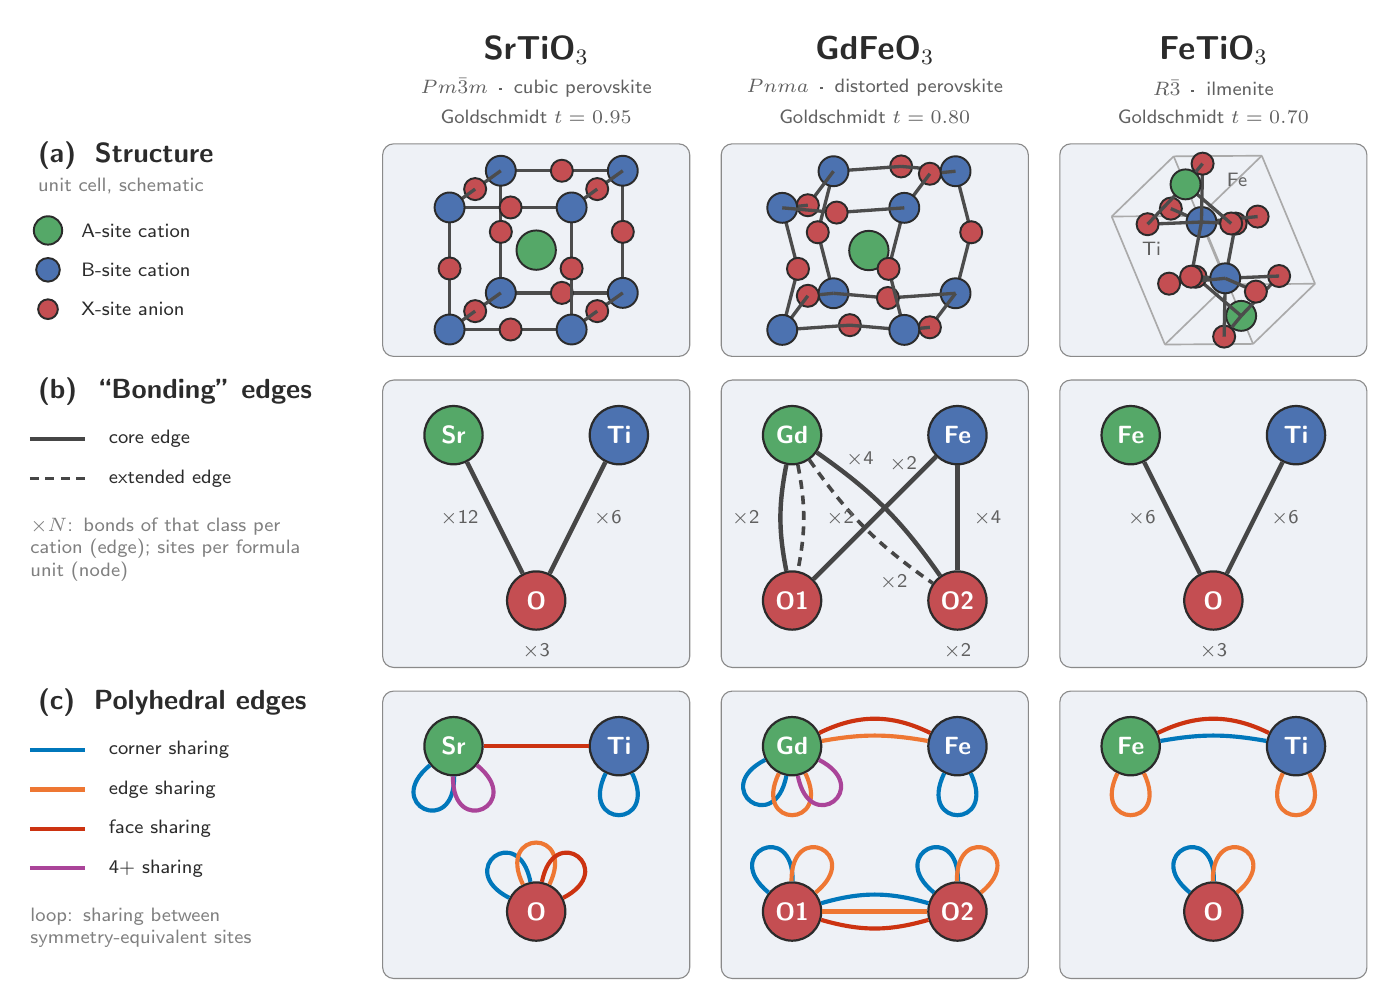
\begin{tikzpicture}

% =====================================================================
%  Geometry bookkeeping (cm)
%    legend column at x = -4.85 .. -0.7 ; material columns at
%    x0 = 0, 4.3, 8.6 ; panel x = x0-0.35 .. x0+3.55 (inner width 3.9)
%  Rows (absolute y):  header 10.55 / 10.91 / 11.38 ;
%    (a) motif    7.50 .. 10.20   (scope shift y = 7.65)
%    (b) bonding  3.55 ..  7.20   (scope shift y = 3.95)
%    (c) poly    -0.40 ..  3.25   (scope shift y = 0)
%  Row (b)/(c) graph panels share one node layout: cations top
%  (y = 2.55), anions bottom (y = 0.45), so the eye maps nodes across rows.
% =====================================================================

% ---------------------------------------------------------------------
%  Column headers
% ---------------------------------------------------------------------
\foreach \x/\formula/\proto/\tf in {%
    1.6/{SrTiO$_3$}/{$Pm\bar3m$ \,·\, cubic perovskite}/{0.95},
    5.9/{GdFeO$_3$}/{$Pnma$ \,·\, distorted perovskite}/{0.80},
    10.2/{FeTiO$_3$}/{$R\bar3$ \,·\, ilmenite}/{0.70}}{
  \node[ptitle, font=\large\bfseries\sffamily] at (\x,11.38) {\formula};
  \node[psub] at (\x,10.91) {\proto};
  \node[psub] at (\x,10.55) {Goldschmidt $t=\tf$};
}

% ---------------------------------------------------------------------
%  Row 1 — structure motifs (3-D ball-and-stick, oblique projection;
%  GENERATED by gen_motif3d.py (this directory) — edit that script, not this block)
% ---------------------------------------------------------------------
% SrTiO3: cubic cell, straight B-O-B cage, A at body centre
\begin{scope}[shift={(0,7.65)}]
  \draw[panelbox] (-0.35,-0.15) rectangle (3.55,2.55);
  \draw[mbond] (1.151,0.657) -- (1.926,0.657);
  \draw[mbond] (1.926,0.657) -- (2.700,0.657);
  \draw[mbond] (1.151,2.208) -- (1.926,2.208);
  \draw[mbond] (1.926,2.208) -- (2.700,2.208);
  \draw[mbond] (1.151,0.657) -- (1.151,1.432);
  \draw[mbond] (1.151,1.432) -- (1.151,2.208);
  \draw[mbond] (2.700,0.657) -- (2.700,1.432);
  \draw[mbond] (2.700,1.432) -- (2.700,2.208);
  \node[matomO] at (1.926,0.657) {};
  \node[matomO] at (1.926,2.208) {};
  \node[matomO] at (1.151,1.432) {};
  \node[matomO] at (2.700,1.432) {};
  \node[matomB] at (1.151,0.657) {};
  \node[matomB] at (1.151,2.208) {};
  \node[matomB] at (2.700,0.657) {};
  \node[matomB] at (2.700,2.208) {};
  \draw[mbond] (0.825,0.425) -- (1.151,0.657);
  \draw[mbond] (2.375,0.425) -- (2.700,0.657);
  \draw[mbond] (0.825,1.975) -- (1.151,2.208);
  \draw[mbond] (2.375,1.975) -- (2.700,2.208);
  \node[matomO] at (0.825,0.425) {};
  \node[matomO] at (2.375,0.425) {};
  \node[matomO] at (0.825,1.975) {};
  \node[matomO] at (2.375,1.975) {};
  \node[matomA] at (1.600,1.200) {};
  \draw[mbond] (0.500,0.192) -- (0.825,0.425);
  \draw[mbond] (2.050,0.192) -- (2.375,0.425);
  \draw[mbond] (0.500,1.742) -- (0.825,1.975);
  \draw[mbond] (2.050,1.742) -- (2.375,1.975);
  \draw[mbond] (0.500,0.192) -- (1.275,0.192);
  \draw[mbond] (1.275,0.192) -- (2.050,0.192);
  \draw[mbond] (0.500,1.742) -- (1.275,1.742);
  \draw[mbond] (1.275,1.742) -- (2.050,1.742);
  \draw[mbond] (0.500,0.192) -- (0.500,0.967);
  \draw[mbond] (0.500,0.967) -- (0.500,1.742);
  \draw[mbond] (2.050,0.192) -- (2.050,0.967);
  \draw[mbond] (2.050,0.967) -- (2.050,1.742);
  \node[matomO] at (1.275,0.192) {};
  \node[matomO] at (1.275,1.742) {};
  \node[matomO] at (0.500,0.967) {};
  \node[matomO] at (2.050,0.967) {};
  \node[matomB] at (0.500,0.192) {};
  \node[matomB] at (0.500,1.742) {};
  \node[matomB] at (2.050,0.192) {};
  \node[matomB] at (2.050,1.742) {};
\end{scope}
% GdFeO3: edge O tangentially displaced (octahedral tilt)
\begin{scope}[shift={(4.3,7.65)}]
  \draw[panelbox] (-0.35,-0.15) rectangle (3.55,2.55);
  \node[matomO] at (1.935,2.263) {};
  \draw[mbond] (1.076,2.202) -- (1.935,2.263);
  \draw[mbond] (1.935,2.263) -- (2.626,2.202);
  \draw[mbond] (1.076,0.652) -- (0.876,1.427);
  \draw[mbond] (0.876,1.427) -- (1.076,2.202);
  \draw[mbond] (2.626,0.652) -- (2.825,1.427);
  \draw[mbond] (2.825,1.427) -- (2.626,2.202);
  \node[matomO] at (0.876,1.427) {};
  \node[matomO] at (2.825,1.427) {};
  \node[matomB] at (1.076,0.652) {};
  \node[matomB] at (1.076,2.202) {};
  \node[matomB] at (2.626,0.652) {};
  \node[matomB] at (2.626,2.202) {};
  \draw[mbond] (1.076,0.652) -- (1.767,0.592);
  \draw[mbond] (1.767,0.592) -- (2.626,0.652);
  \node[matomO] at (1.767,0.592) {};
  \draw[mbond] (0.750,0.620) -- (1.076,0.652);
  \draw[mbond] (2.300,0.220) -- (2.626,0.652);
  \draw[mbond] (0.750,1.770) -- (1.076,2.202);
  \draw[mbond] (2.300,2.170) -- (2.626,2.202);
  \node[matomO] at (0.750,0.620) {};
  \node[matomO] at (2.300,0.220) {};
  \node[matomO] at (0.750,1.770) {};
  \node[matomO] at (2.300,2.170) {};
  \node[matomA] at (1.525,1.195) {};
  \draw[mbond] (0.425,0.187) -- (0.750,0.620);
  \draw[mbond] (1.975,0.187) -- (2.300,0.220);
  \draw[mbond] (0.425,1.737) -- (0.750,1.770);
  \draw[mbond] (1.975,1.737) -- (2.300,2.170);
  \node[matomO] at (1.284,0.247) {};
  \draw[mbond] (0.425,0.187) -- (1.284,0.247);
  \draw[mbond] (1.284,0.247) -- (1.975,0.187);
  \draw[mbond] (0.425,0.187) -- (0.625,0.962);
  \draw[mbond] (0.625,0.962) -- (0.425,1.737);
  \draw[mbond] (1.975,0.187) -- (1.775,0.962);
  \draw[mbond] (1.775,0.962) -- (1.975,1.737);
  \node[matomO] at (0.625,0.962) {};
  \node[matomO] at (1.775,0.962) {};
  \node[matomB] at (0.425,0.187) {};
  \node[matomB] at (0.425,1.737) {};
  \node[matomB] at (1.975,0.187) {};
  \node[matomB] at (1.975,1.737) {};
  \draw[mbond] (0.425,1.737) -- (1.116,1.677);
  \draw[mbond] (1.116,1.677) -- (1.975,1.737);
  \node[matomO] at (1.116,1.677) {};
\end{scope}
% FeTiO3: primitive rhombohedral cell, oblique view (orientation
% sweep option Q): the two face-sharing Fe-Ti pairs along the body
% diagonal with the shared O3 triangles shown in depth
\begin{scope}[shift={(8.6,7.65)}]
  \draw[panelbox] (-0.35,-0.15) rectangle (3.55,2.55);
  \draw[medge] (2.104,0.009) -- (2.891,0.773);
  \draw[medge] (2.104,0.009) -- (0.985,0.001);
  \draw[medge] (2.104,0.009) -- (1.427,1.635);
  \draw[medge] (2.891,0.773) -- (1.773,0.765);
  \draw[medge] (2.891,0.773) -- (2.215,2.399);
  \draw[medge] (0.985,0.001) -- (1.773,0.765);
  \draw[medge] (0.985,0.001) -- (0.309,1.627);
  \draw[medge] (1.427,1.635) -- (2.215,2.399);
  \draw[medge] (1.427,1.635) -- (0.309,1.627);
  \draw[medge] (1.773,0.765) -- (1.096,2.391);
  \draw[medge] (2.215,2.399) -- (1.096,2.391);
  \draw[medge] (0.309,1.627) -- (1.096,2.391);
  \node[matomA, minimum size=3.8mm] at (1.953,0.365) {};
  \draw[mbond] (1.953,0.365) -- (2.435,0.871);
  \node[matomO] at (2.435,0.871) {};
  \draw[mbond] (1.953,0.365) -- (1.374,0.862);
  \node[matomO] at (1.374,0.862) {};
  \draw[mbond] (1.953,0.365) -- (1.737,0.102);
  \draw[mbond] (1.751,0.842) -- (2.435,0.871);
  \draw[mbond] (1.751,0.842) -- (1.374,0.862);
  \node[matomO] at (1.883,1.537) {};
  \draw[mbond] (1.751,0.842) -- (1.883,1.537);
  \node[matomO] at (1.737,0.102) {};
  \draw[mbond] (1.751,0.842) -- (1.737,0.102);
  \node[matomB] at (1.751,0.842) {};
  \draw[mbond] (1.751,0.842) -- (2.140,0.673);
  \draw[mbond] (1.751,0.842) -- (1.038,0.774);
  \node[matomO] at (2.140,0.673) {};
  \node[matomO] at (1.038,0.774) {};
  \node[matomO] at (2.162,1.626) {};
  \node[matomO] at (1.060,1.727) {};
  \draw[mbond] (1.449,1.557) -- (2.162,1.626);
  \draw[mbond] (1.449,1.557) -- (1.060,1.727);
  \node[matomB] at (1.449,1.557) {};
  \draw[mbond] (1.449,1.557) -- (1.463,2.298);
  \node[matomO] at (1.463,2.298) {};
  \draw[mbond] (1.449,1.557) -- (1.317,0.863);
  \node[matomO] at (1.317,0.863) {};
  \draw[mbond] (1.449,1.557) -- (1.826,1.538);
  \draw[mbond] (1.449,1.557) -- (0.765,1.529);
  \draw[mbond] (1.247,2.035) -- (1.463,2.298);
  \node[matomO] at (1.826,1.538) {};
  \draw[mbond] (1.247,2.035) -- (1.826,1.538);
  \node[matomO] at (0.765,1.529) {};
  \draw[mbond] (1.247,2.035) -- (0.765,1.529);
  \node[matomA, minimum size=3.8mm] at (1.247,2.035) {};
  \node[psub, anchor=west] at (-0.457+2.104,2.086+0.009) {Fe};
  \node[psub, anchor=east] at (-1.045+2.104,1.208+0.009) {Ti};
\end{scope}

% ---------------------------------------------------------------------
%  Row 2 — bonding edges (condensed graphs)
%  node layout: cations top, anions bottom (identical in row 3)
% ---------------------------------------------------------------------
% ---- SrTiO3 : Sr-O core, Ti-O core ----------------------------------
\begin{scope}[shift={(0,3.95)}]
  \draw[panelbox] (-0.35,-0.40) rectangle (3.55,3.25);
  \node[siteA] (Sr) at (0.55,2.55) {Sr};
  \node[siteB] (Ti) at (2.65,2.55) {Ti};
  \node[siteO] (O)  at (1.60,0.45) {O};
  \draw[core] (Sr) -- (O);
  \draw[core] (Ti) -- (O);
  % bond multiplicities (bonds of this class per cation; builder mp-5229)
  \node[psub, anchor=east] at (0.99,1.50) {$\times$12};
  \node[psub, anchor=west] at (2.21,1.50) {$\times$6};
  % site multiplicity: 3 equivalent O per formula unit
  \node[psub, anchor=north] at (1.60,0.02) {$\times$3};
\end{scope}
% ---- GdFeO3 : Fe-O1, Fe-O2 core ; Gd-O1, Gd-O2 core+extended --------
\begin{scope}[shift={(4.3,3.95)}]
  \draw[panelbox] (-0.35,-0.40) rectangle (3.55,3.25);
  \node[siteA] (Gd) at (0.55,2.55) {Gd};
  \node[siteB] (Fe) at (2.65,2.55) {Fe};
  \node[siteO] (Oa) at (0.55,0.45) {O1};
  \node[siteO] (Ob) at (2.65,0.45) {O2};
  \draw[core] (Gd) to[bend right=11] (Oa);
  \draw[ext]  (Gd) to[bend left=11]  (Oa);
  \draw[core] (Gd) to[bend left=10]  (Ob);
  \draw[ext]  (Gd) to[bend right=10] (Ob);
  \draw[core] (Fe) -- (Oa);
  \draw[core] (Fe) -- (Ob);
  % bond multiplicities (bonds of this class per cation; builder mp-600576:
  % O1 = apical 4c, O2 = equatorial 8d; Gd core 2+4, ext 2+2; Fe 2+4)
  \node[psub, anchor=east]  at (0.26,1.50) {$\times$2};  % Gd-O1 core (left bulge)
  \node[psub, anchor=west]  at (0.86,1.50) {$\times$2};  % Gd-O1 ext (right bulge)
  \node[psub, anchor=south] at (1.41,2.02) {$\times$4};  % Gd-O2 core (upper bulge)
  \node[psub, anchor=north] at (1.84,0.90) {$\times$2};  % Gd-O2 ext (lower bulge)
  \node[psub, anchor=east]  at (2.26,2.18) {$\times$2};  % Fe-O1 (near Fe end)
  \node[psub, anchor=west]  at (2.73,1.50) {$\times$4};  % Fe-O2
  % site multiplicity: O2 = 8d, 2 sites per formula unit (O1 = 4c, 1)
  \node[psub, anchor=north] at (2.65,0.02) {$\times$2};
\end{scope}
% ---- FeTiO3 : Fe-O core, Ti-O core ----------------------------------
\begin{scope}[shift={(8.6,3.95)}]
  \draw[panelbox] (-0.35,-0.40) rectangle (3.55,3.25);
  \node[siteA] (Fe) at (0.55,2.55) {Fe};
  \node[siteB] (Ti) at (2.65,2.55) {Ti};
  \node[siteO] (O)  at (1.60,0.45) {O};
  \draw[core] (Fe) -- (O);
  \draw[core] (Ti) -- (O);
  % bond multiplicities (bonds of this class per cation; builder mp-19417)
  \node[psub, anchor=east] at (0.99,1.50) {$\times$6};
  \node[psub, anchor=west] at (2.21,1.50) {$\times$6};
  % site multiplicity: 3 equivalent O per formula unit
  \node[psub, anchor=north] at (1.60,0.02) {$\times$3};
\end{scope}

% ---------------------------------------------------------------------
%  Row 3 — polyhedral edges (condensed graphs, same node layout)
% ---------------------------------------------------------------------
% ---- SrTiO3 ---------------------------------------------------------
\begin{scope}[shift={(0,0)}]
  \draw[panelbox] (-0.35,-0.40) rectangle (3.55,3.25);
  \node[siteA] (Sr) at (0.55,2.55) {Sr};
  \node[siteB] (Ti) at (2.65,2.55) {Ti};
  \node[siteO] (O)  at (1.60,0.45) {O};
  \draw[pface] (Sr) -- (Ti);
  \gcloop{pcorner}{Sr}{245}
  \gcloop{pmulti}{Sr}{295}
  \gcloop{pcorner}{Ti}{270}
  \gcloop{pcorner}{O}{127}
  \gcloop{pedge}{O}{90}
  \gcloop{pface}{O}{53}
\end{scope}
% ---- GdFeO3 ---------------------------------------------------------
\begin{scope}[shift={(4.3,0)}]
  \draw[panelbox] (-0.35,-0.40) rectangle (3.55,3.25);
  \node[siteA] (Gd) at (0.55,2.55) {Gd};
  \node[siteB] (Fe) at (2.65,2.55) {Fe};
  \node[siteO] (Oa) at (0.55,0.45) {O1};
  \node[siteO] (Ob) at (2.65,0.45) {O2};
  \draw[pedge] (Gd) to[bend left=10] (Fe);
  \draw[pface] (Gd) to[bend left=26] (Fe);
  \draw[pcorner] (Oa) to[bend left=16] (Ob);
  \draw[pedge]   (Oa) -- (Ob);
  \draw[pface]   (Oa) to[bend right=16]  (Ob);
  \gcloop{pcorner}{Gd}{233}
  \gcloop{pedge}{Gd}{270}
  \gcloop{pmulti}{Gd}{307}
  \gcloop{pcorner}{Fe}{270}
  \gcloop{pcorner}{Oa}{115}
  \gcloop{pedge}{Oa}{65}
  \gcloop{pcorner}{Ob}{115}
  \gcloop{pedge}{Ob}{65}
\end{scope}
% ---- FeTiO3 ---------------------------------------------------------
\begin{scope}[shift={(8.6,0)}]
  \draw[panelbox] (-0.35,-0.40) rectangle (3.55,3.25);
  \node[siteA] (Fe) at (0.55,2.55) {Fe};
  \node[siteB] (Ti) at (2.65,2.55) {Ti};
  \node[siteO] (O)  at (1.60,0.45) {O};
  \draw[pcorner] (Fe) to[bend left=10] (Ti);
  \draw[pface]   (Fe) to[bend left=26] (Ti);
  \gcloop{pedge}{Fe}{270}
  \gcloop{pedge}{Ti}{270}
  \gcloop{pcorner}{O}{115}
  \gcloop{pedge}{O}{65}
\end{scope}

% ---------------------------------------------------------------------
%  Legend column (x ~ -4.85 .. -0.7): row tags (a)/(b)/(c) + keys.
%  Definitions (condensation rule, x N notation) live in the caption.
% ---------------------------------------------------------------------
\begin{scope}[shift={(-4.85,0)}]
  % ---- (a) structure ----
  \node[rowlbl] at (0,10.05) {(a)\; Structure};
  \node[rowlbl, text=ink!60, font=\scriptsize\sffamily] at (0,9.67) {unit cell, schematic};
  \node[matomA, minimum size=3.6mm] at (0.25,9.10) {}; \node[leglbl] at (0.55,9.10) {A-site cation};
  \node[matomB, minimum size=3.0mm] at (0.25,8.60) {}; \node[leglbl] at (0.55,8.60) {B-site cation};
  \node[matomO, minimum size=2.5mm] at (0.25,8.10) {}; \node[leglbl] at (0.55,8.10) {X-site anion};

  % ---- (b) bonding edges ----
  \node[rowlbl] at (0,7.05) {(b)\; ``Bonding'' edges};
  \draw[core] (0.02,6.45) -- (0.72,6.45); \node[leglbl] at (0.90,6.45) {core edge};
  \draw[ext]  (0.02,5.95) -- (0.72,5.95); \node[leglbl] at (0.90,5.95) {extended edge};
  \node[leghint] at (0.02,5.45)
    {$\times N$: bonds of that class per cation (edge); sites per formula unit (node)};

  % ---- (c) polyhedral edges ----
  \node[rowlbl] at (0,3.10) {(c)\; Polyhedral edges};
  \draw[pcorner] (0.02,2.50) -- (0.72,2.50); \node[leglbl] at (0.90,2.50) {corner sharing};
  \draw[pedge]   (0.02,2.00) -- (0.72,2.00); \node[leglbl] at (0.90,2.00) {edge sharing};
  \draw[pface]   (0.02,1.50) -- (0.72,1.50); \node[leglbl] at (0.90,1.50) {face sharing};
  \draw[pmulti]  (0.02,1.00) -- (0.72,1.00); \node[leglbl] at (0.90,1.00) {4+ sharing};
  \node[leghint] at (0.02,0.50)
    {loop: sharing between symmetry-equivalent sites};
\end{scope}

\end{tikzpicture}
\endgroup
